% Compilazione: pdflatex -jobname=ottica_tex ottica.tex
\documentclass[11pt,a4paper]{article}
\usepackage[utf8]{inputenc}\usepackage[T1]{fontenc}\IfFileExists{italian.ldf}{\usepackage[italian]{babel}}{\usepackage[english]{babel}}
\usepackage{amsmath,amssymb,geometry,graphicx,tikz}\geometry{margin=2cm}
\setlength{\parindent}{0pt}\setlength{\parskip}{5pt}
\newcommand{\pagina}[1]{\clearpage}
\newcommand{\vv}[1]{\vec{#1}}
\begin{document}
% Pagina originale 1
\section*{Ottica -- Legenda}
1. Onde elettromagnetiche: operatori differenziali; teoremi della divergenza e di Stokes; equazioni di Maxwell; dielettrici; fenomeni oscillatori e ondulatori; analisi di Fourier; fronte d'onda; onde sferiche e sonore; sovrapposizione di onde; ampiezza massima e minima di un'onda stazionaria; orecchio umano; effetto Doppler, autovelox ed eco Doppler; onde elettromagnetiche e loro proprietà; onde di propagazione generale e piane; onde nei dielettrici; vettore di Poynting; tipi e produzione di onde EM; polarizzazione; lamine polarizzatrici.

2. Riflessione e rifrazione: riflessione; rifrazione; condizioni di raccordo; angolo limite; energia; incidenza normale; angolo di Brewster; passaggio nei materiali; principio di Fermat; attraversamento di lamina piana; effetti visivi della rifrazione; angolo di deviazione.

3. Ottica geometrica: elemento ottico; specchi concavo e convesso; convenzione dei segni; costruzione dell'immagine; ingrandimento trasversale; specchio piano; diottro; costruzione dell'immagine; diottri piani; lenti; lente sottile; classificazione; lenti convergenti e divergenti; costruzione dell'immagine; ingrandimento; sistema di lenti; occhio; immagini reali e virtuali.

4. Interferenza e diffrazione: interferenza; esperimento di Young; sorgenti incoerenti; effetto cromatico; lamina sottile; cuneo sottile; anelli di Newton; interferenza di $N$ sorgenti; caratteristiche; diffrazione; diffrazione di Fraunhofer da fenditura singola; apertura circolare; criterio di Rayleigh; interferenza e diffrazione; caso di $N$ sorgenti.

5. Formule utili.
% Pagina originale 2
\pagina{2}\section*{Operatori differenziali}
Sia $f:\mathbb R^n\to\mathbb R$ una funzione scalare ($n=3$ caso spaziale).
\[\vv\nabla f=\operatorname{grad}f=\frac{\partial f}{\partial x}\hat u_x+\frac{\partial f}{\partial y}\hat u_y+\frac{\partial f}{\partial z}\hat u_z\in\mathbb R^n.\]
Operatore nabla: $\vv\nabla=(\partial_x,\partial_y,\partial_z)$, con $n=3$.
Sia $\vv F:\mathbb R^n\to\mathbb R^n$ una funzione vettoriale (campo).
\[\vv\nabla\cdot\vv F=\frac{\partial F_x}{\partial x}+\frac{\partial F_y}{\partial y}+\frac{\partial F_z}{\partial z}\in\mathbb R\quad\text{(divergenza, scalare)}.\]
\[\vv\nabla\times\vv F=\begin{vmatrix}\hat u_x&\hat u_y&\hat u_z\\\partial_x&\partial_y&\partial_z\\F_x&F_y&F_z\end{vmatrix}
=\left(\partial_yF_z-\partial_zF_y,\partial_zF_x-\partial_xF_z,\partial_xF_y-\partial_yF_x\right)\in\mathbb R^3.\]
Rotore: $\operatorname{rot}\vv F$. Teorema della divergenza:
\[\oint_\Sigma\vv F\cdot d\vv\Sigma=\int_\tau(\vv\nabla\cdot\vv F)\,d\tau,\]
$\Sigma$ superficie chiusa, $\tau$ volume racchiuso. Teorema di Stokes:
\[\oint_s\vv F\cdot d\vv s=\int_\Sigma(\vv\nabla\times\vv F)\cdot d\vv\Sigma.\]
$s$ contorno (circolazione), $\Sigma$ superficie, $d\vv\Sigma=\hat u_n d\Sigma$.
\[\operatorname{rot}(\operatorname{grad}f)\in\mathbb R^3,\quad\operatorname{div}(\operatorname{grad}f)\in\mathbb R,\quad\operatorname{div}(\operatorname{rot}\vv F)\in\mathbb R,\quad\operatorname{grad}(\operatorname{div}\vv F)\in\mathbb R^3.\]
$\vv\nabla\times(\vv\nabla\cdot\vv F)$ e $\vv\nabla(\vv\nabla\times\vv F)$ non hanno senso nelle operazioni indicate.
\[\vv\nabla\cdot\vv\nabla f=\nabla^2f\quad\text{(laplaciano)},\qquad\vv\nabla\times\vv\nabla f=0,\qquad\vv\nabla\cdot(\vv\nabla\times\vv F)=0.\]
\[\vv\nabla\times(\vv\nabla\times\vv F)=\vv\nabla(\vv\nabla\cdot\vv F)-\nabla^2\vv F.\]
% Pagina originale 3
\pagina{3}\section*{Equazioni di Maxwell}
Campo elettrostatico conservativo:
\[\oint_s\vv E\cdot d\vv s=0=\int_\Sigma(\vv\nabla\times\vv E)\cdot d\vv\Sigma\implies\vv\nabla\times\vv E=0.\]
Legge di Gauss:
\[\Phi_E=\oint_\Sigma\vv E\cdot d\vv\Sigma=\frac{q}{\epsilon_0}=\frac1{\epsilon_0}\int_\tau\rho\,d\tau.\]
\[\oint_\Sigma\vv E\cdot d\vv\Sigma=\int_\tau(\vv\nabla\cdot\vv E)\,d\tau=\int_\tau\frac\rho{\epsilon_0}\,d\tau\implies\vv\nabla\cdot\vv E=\frac\rho{\epsilon_0}.\]
Non esistono monopoli magnetici: $\vv\nabla\cdot\vv B=0$.
Legge di Ampère:
\[\oint_s\vv B\cdot d\vv s=\mu_0i=\mu_0\int_\Sigma\vv j\cdot d\vv\Sigma=\int_\Sigma(\vv\nabla\times\vv B)\cdot d\vv\Sigma\implies\vv\nabla\times\vv B=\mu_0\vv j.\]
In condizioni stazionarie:
\[\vv\nabla\cdot\vv E=\rho/\epsilon_0,\quad\vv\nabla\times\vv E=0,\quad\vv\nabla\cdot\vv B=0,\quad\vv\nabla\times\vv B=\mu_0\vv j.\]
Legge di Faraday--Lenz:
\[\mathcal E_i=-\frac{\partial\Phi_B}{\partial t}=-\frac\partial{\partial t}\int_\Sigma\vv B\cdot d\vv\Sigma=-\int_\Sigma\frac{\partial\vv B}{\partial t}\cdot d\vv\Sigma.\]
\[\oint_s\vv E_i\cdot d\vv s=\int_\Sigma(\vv\nabla\times\vv E)\cdot d\vv\Sigma
\implies\vv\nabla\times\vv E=-\frac{\partial\vv B}{\partial t}.\]
In condizioni stazionarie $\oint_\Sigma\vv j\cdot d\vv\Sigma=0$; in condizioni non stazionarie $\oint_\Sigma\vv j\cdot d\vv\Sigma=-dq/dt$ (equazione di continuità).
Schema del condensatore: in regime stazionario le correnti sui due lati sono $i,i$; in regime non stazionario $i\ne i'$, $i'=i+i_s$, con $i_s$ corrente di spostamento.
% Pagina originale 4
\pagina{4}
\[i_s=\int_\Sigma\vv j_s\cdot d\vv\Sigma=\epsilon_0\frac{d\Phi_E}{dt},\qquad\vv J_{\rm tot}=\vv J+\epsilon_0\frac{\partial\vv E}{\partial t}.\]
$\vv J$: densità di corrente ordinaria; $\vv J_s=\epsilon_0\partial_t\vv E$: densità di corrente di spostamento.
Nuova legge di Ampère:
\[\oint_s\vv B\cdot d\vv s=\mu_0(i+i_s)\implies\vv\nabla\times\vv B=\mu_0\left(\vv j+\epsilon_0\frac{\partial\vv E}{\partial t}\right).\]
In condizioni non stazionarie:
\[\vv\nabla\cdot\vv E=\rho/\epsilon_0,\quad\vv\nabla\times\vv E=-\partial_t\vv B,\quad\vv\nabla\cdot\vv B=0,\quad\vv\nabla\times\vv B=\mu_0(\vv j+\epsilon_0\partial_t\vv E).\]
\section*{Dielettrici}
Materiali non conduttori. $\Delta V<\Delta V_0$ (con il dielettrico rispetto al vuoto).
\[k=\frac{\Delta V_0}{\Delta V}>1\quad\text{costante dielettrica relativa (permittività elettrica)}.\]
\[\Delta E=E_0-E_k=\frac{\sigma_0}{\epsilon_0}-\frac{\sigma_0}{k\epsilon_0}=\frac{k-1}{k}\frac{\sigma_0}{\epsilon_0}=\frac\chi{\chi+1}\frac{\sigma_0}{\epsilon_0},\quad\chi=k-1.\]
$\chi$: suscettività elettrica; $\epsilon=\epsilon_0k$.
\[\vv P=\epsilon_0(k-1)\vv E=\epsilon_0\chi\vv E\quad\text{vettore polarizzazione};\]
\[\vv D=\epsilon_0\vv E+\vv P=\epsilon_0(\chi+1)\vv E=\epsilon_0k\vv E=\epsilon\vv E\quad\text{induzione dielettrica}.\]
\[\Delta B=B-B_0=(k_m-1)B_0=\chi_m B_0,\quad\vv M=\chi_mni,\quad\vv H=ni.\]
$\vv M$: campo di magnetizzazione; $\vv H$: campo magnetico esterno; $k_m$ permittività magnetica, $\chi_m$ suscettività magnetica; negli appunti $k_m=B/B_0<1$.
\[\vv B=\mu_0(\vv H+\vv M)=\mu_0(\chi_m+1)\vv H=\mu_0k_m\vv H=\mu\vv H.\]
\[\vv\nabla\cdot\vv D=\rho_l,\quad\vv\nabla\times\vv E=-\partial_t\vv B,\quad\vv\nabla\cdot\vv B=0,\quad\vv\nabla\times\vv H=\vv j+\partial_t\vv D.\]
% Pagina originale 5
\pagina{5}\section*{Fenomeni oscillatori}
Oscillazione: un movimento periodico di un sistema attorno ad una posizione di equilibrio.
\[x(t)=A\cos(\omega t+\varphi),\quad\omega=2\pi f,\quad f=T^{-1}=1/T\ [\mathrm{Hz}].\]
Oscillatore armonico semplice: il grafico sinusoidale ha ampiezza $A$ e periodo $T$; valore iniziale $A\cos\varphi$.
Esempio, moto armonico semplice:
\[-kx=m\frac{d^2x}{dt^2}\implies x(t)=A\sin(\omega t+\varphi),\]
\[x'(t)=A\omega\cos(\omega t+\varphi)=v(t),\quad x''(t)=-A\omega^2\sin(\omega t+\varphi)=a(t)=-\omega^2x(t).\]
L'energia nel moto armonico semplice senza smorzamento è costante: $E=E_p+E_k$.
\[E_p=\tfrac12kx^2,\quad E_k=\tfrac12mv^2,\quad\omega=\sqrt{k/m},\quad k=m\omega^2.\]
\[E=\tfrac12kA^2\sin^2(\omega t+\varphi)+\tfrac12m\omega^2A^2\cos^2(\omega t+\varphi)=\tfrac12kA^2[\sin^2(\omega t+\varphi)+\cos^2(\omega t+\varphi)]=\tfrac12kA^2.\]
Vale il principio di sovrapposizione degli effetti (PSE):
\[x_1=A_1\cos\omega t,\quad x_2=A_2\cos(\omega t+\varphi)\implies x=A\cos(\omega t+\psi),\]
\[A=\sqrt{A_1^2+A_2^2+2A_1A_2\cos\varphi}\quad\text{(teorema di Carnot)}.\]
% Pagina originale 6
\pagina{6}
Più generalmente:
\[x(t)=x_1(t)+x_2(t)=A_1\cos(\omega_1t+\varphi_1)+A_2\cos(\omega_2t+\varphi_2).\]
Per ampiezze uguali e fasi nulle:
\[x(t)=2A\cos\left(\frac{\omega_2-\omega_1}{2}t\right)\cos\left(\frac{\omega_1+\omega_2}{2}t\right)=2A\cos\Omega t\cos\omega t,\]
\[\Omega=(\omega_2-\omega_1)/2,\qquad\omega=(\omega_1+\omega_2)/2.\]
Grafico: ampiezza modulata con pulsazione $\Omega$, oscillazioni interne con pulsazione $\omega$.
Con smorzamento: $f_{\rm att}=-\lambda v$, $A_2<A_1$, $A_i<A_{i-1}$ per ogni $i>0$.
\[-kx-\lambda v=ma\implies\frac{d^2x}{dt^2}+\frac\lambda m\frac{dx}{dt}+\frac kmx=0.\]
Definito il coefficiente di smorzamento $\gamma=\lambda/(2m)$:
\[x''+2\gamma x'+\omega_0^2x=0,\qquad x(t)=c_1e^{z_1t}+c_2e^{z_2t}.\]
\begin{align*}
\Delta>0\ (\gamma^2>\omega_0^2):&\quad x=e^{-\gamma t}\left(c_1e^{\sqrt{\gamma^2-\omega_0^2}t}+c_2e^{-\sqrt{\gamma^2-\omega_0^2}t}\right),\\
\Delta=0\ (\gamma^2=\omega_0^2):&\quad x=Ae^{-\gamma t}(c_1+c_2t),\\
\Delta<0\ (\gamma^2<\omega_0^2):&\quad x=Ae^{-\gamma t}\cos\left(\sqrt{\omega_0^2-\gamma^2}t+\psi\right).
\end{align*}
Rispettivamente: smorzamento forte, critico, debole. Il grafico confronta decadimento monotono e oscillazioni smorzate fra gli inviluppi esponenziali.
% Pagina originale 7
\pagina{7}\section*{Fenomeni ondulatori}
Sono perturbazioni prodotte da una sorgente caratterizzate da una propagazione di energia meccanica e quantità di moto senza trasferimento di materia.
\[y(x,t)=A\cos(kx-\omega t+\varphi),\]
$k$ numero d'onda; $\omega$ frequenza angolare; $\varphi$ sfasamento iniziale.
Due tipi: meccaniche (si propagano solo in mezzi materiali) ed elettromagnetiche (si propagano anche nel vuoto).
Per direzione: longitudinali (vibrazione parallela alla propagazione), trasversali (vibrazione perpendicolare alla propagazione).
Unidimensionali: lungo una retta; bidimensionali: in un piano; tridimensionali: nello spazio.
Tutti i fenomeni ondulatori soddisfano l'equazione di d'Alembert:
\[\frac{\partial^2\xi}{\partial t^2}=v^2\frac{\partial^2\xi}{\partial x^2},\]
$\xi$ perturbazione del punto materiale; $v$ velocità di propagazione dell'onda nel mezzo. Soluzione indicata: $\xi(x\pm vt)$. Verifica ponendo $u=x-vt$.
% Pagina originale 8
\pagina{8}
\begin{align*}
\partial_x\xi(x-vt)&=\frac{d\xi}{du}\partial_xu=\xi'(u),\\
\partial_x^2\xi(x-vt)&=\frac{d\xi'}{du}\partial_xu=\xi''(u),\\
\partial_t\xi(x-vt)&=\frac{d\xi}{du}\partial_tu=-v\xi'(u),\\
\partial_t^2\xi(x-vt)&=-v\frac{d\xi'}{du}\partial_tu=v^2\xi''(u)=v^2\partial_x^2\xi.
\end{align*}
Onde progressive: impulso che avanza verso $+x$; regressive: verso $-x$.
\begin{align*}v_x&=\frac{dx}{dt}\quad\text{velocità di propagazione dell'onda},\\ v_\xi&=\frac{\partial\xi}{\partial t}\quad\text{velocità di oscillazione delle particelle del mezzo}.\end{align*}
Vale il PSE: $\xi(x,t)=a\xi_1(x,t)+b\xi_2(x,t)$.
\[k=\omega/v=2\pi/\lambda,\quad v=\omega/k,\quad\lambda=2\pi/k,\quad T=2\pi/\omega,\quad\lambda=vT,\quad v=\lambda f.\]
Nei grafici sinusoidali: $\lambda$ è il periodo spaziale e $T$ quello temporale.
% Pagina originale 9
\pagina{9}\section*{Analisi di Fourier}
Ogni segnale in funzione del tempo può essere rappresentato come somma di seni aventi ampiezze e frequenze diverse:
\[\sigma=\sum_i A_i\sin(\omega_it+\varphi_i).\]
Una generica funzione $f$ periodica è rappresentabile come
\[f(t)=a_0+\sum_{m=1}^\infty\left(a_m\sin m\omega t+b_m\cos m\omega t\right),\]
$a_0$ valore medio nel periodo,
\[a_m=\frac2T\int_0^Tf(t)\sin m\omega t\,dt,\qquad b_m=\frac2T\int_0^Tf(t)\cos m\omega t\,dt.\]
\section*{Fronte d'onda}
Luogo dei punti caratterizzati dal medesimo stato di vibrazione.
\[\vv k=\frac{2\pi}\lambda\hat x,\qquad\vv k\cdot\vv r=kx,\qquad\vv k\parallel\vv v\perp\pi.\]
$\pi$ piano del fronte d'onda. Equazione di d'Alembert nello spazio:
\[\partial_t^2\xi=v^2(\partial_x^2\xi+\partial_y^2\xi+\partial_z^2\xi)=v^2\nabla^2\xi.\]
% Pagina originale 10
\pagina{10}\section*{Onde sferiche}
\[\xi(r,t)=A(r)\sin(kr-\omega t),\]
$r$ distanza dalla sorgente $S$; ampiezza variabile. L'intensità varia al variare di $r$:
\[I(r)=cA(r)^2,\qquad I=P/\Sigma=\frac{\text{potenza}}{\text{superficie}}.\]
\[P_m=I\Sigma=cA(r)^2\,4\pi r^2=\text{costante}\implies A(r)\propto1/r.\]
\[A(r)=\xi_0/r\implies\xi(r,t)=\frac{\xi_0}r\sin(kr-\omega t),\qquad I(r)=cA(r)^2=I_0/r^2.\]
\textit{Nota di trascrizione: nell'ultima uguaglianza degli appunti compare anche $\xi_0^2/r^2$, con la costante di proporzionalità sottintesa.}
\section*{Onde sonore}
Onde meccaniche, non si propagano nel vuoto.
\[v_s=\sqrt{\beta/\rho},\]
$\beta$ modulo di compressione $[\mathrm{Pa}]$, $\rho$ densità volumica $[\mathrm{kg/m^3}]$. Nell'aria $v_s$ è $330\div340\ \mathrm{m/s}$; dipende dal materiale (mezzo) e dalla temperatura.
Esempi: a $0^\circ\mathrm C$, $331\ \mathrm{m/s}$; a $20^\circ\mathrm C$, $343\ \mathrm{m/s}$.
L'orecchio è un recettore logaritmico:
\[\mathrm{dB}=10\log_{10}(I/I_0),\qquad I_0=10^{-12}\ \mathrm{W/m^2}\quad\text{soglia di udibilità}.\]
Esempio: $I=10^{-6}\ \mathrm{W/m^2}$ dà $10\log_{10}(I/I_0)=10\cdot6=60\ \mathrm{dB}$.
% Pagina originale 11
\pagina{11}
Il livello sonoro non dipende dalla frequenza, che invece determina se il suono sia acuto o grave.
\section*{Sovrapposizione di onde}
Caso di onde solamente sfasate:
\[\xi_1(x,t)=\xi_0\sin(kx-\omega t),\qquad\xi_2(x,t)=\xi_0\sin(kx-\omega t+\delta).\]
\[\xi_s=\xi_1+\xi_2=\xi_{0s}\sin(kx-\omega t+\psi).\]
Ricordando $\sin\alpha+\sin\beta=2\cos\frac{\alpha-\beta}2\sin\frac{\alpha+\beta}2$, otteniamo
\[\xi_1+\xi_2=\xi_0[\sin(kx-\omega t)+\sin(kx-\omega t+\delta)]
=2\xi_0\cos\frac\delta2\sin\left(kx-\omega t+\frac\delta2\right).\]
$\xi_{0s}=2\xi_0\cos(\delta/2)$, $\psi=\delta/2$.
\[I=cA(r)^2=4c\xi_0^2\cos^2(\delta/2)=4I_0\cos^2(\delta/2),\qquad I_0=c\xi_0^2.\]
$\delta/2=m\pi$, $m\in\mathbb N$: $|I|=4|I_0|$; $\delta/2=(m+\tfrac12)\pi$: $I=0$.
Caso di ampiezza uguale e frequenza diversa:
\[\xi_1=\xi_0\sin(k_1x-\omega_1t),\quad\xi_2=\xi_0\sin(k_2x-\omega_2t),\]
\[\xi_s=2\xi_0\cos\left(\frac{\Delta k}2x-\frac{\Delta\omega}2t\right)\sin(k_mx-\omega_mt).\]
% Pagina originale 12
\pagina{12}
\[\Delta k=k_1-k_2,\quad\Delta\omega=\omega_1-\omega_2,\quad k_m=(k_1+k_2)/2,\quad\omega_m=(\omega_1+\omega_2)/2.\]
\[A(x,t)=2\xi_0\cos\left(\frac{\Delta k}2x-\frac{\Delta\omega}2t\right).\]
L'ampiezza varia nello spazio e nel tempo; velocità di propagazione dell'inviluppo $v_g=\Delta\omega/\Delta k$.
Per un ascoltatore a distanza fissa $x=L$:
\[\xi(L,t)=2\xi_0\cos\left(\frac{\Delta k}2L-\frac{\Delta\omega}2t\right)\sin(k_mL-\omega_mt).\]
Ponendo $\varphi=\Delta kL/2$, $\psi=k_mL$:
\[\xi(L,t)=2\xi_0\cos(\varphi-\Delta\omega t/2)\sin(\psi-\omega_mt).\]
Caso particolare:
\[\xi_1=\xi_0\sin(kx-\omega t),\quad\xi_2=\xi_0\sin(kx+\omega t),\quad\Delta k=0,\quad\omega_m=0,\]
\[\xi(x,t)=2\xi_0\cos(\omega t)\sin(kx)\quad\text{onda stazionaria (OS)}.\]
Ampiezza massima: $2\xi_0\sin(kx)=2\xi_0\sin(2\pi x/\lambda)$; derivando,
\[2\xi_0\cos(2\pi x/\lambda)\frac{2\pi}\lambda=0\iff\frac{2\pi}\lambda x=(m+\tfrac12)\pi\implies x=(m+\tfrac12)\frac\lambda2.\]
Ampiezza minima:
\[2\xi_0\sin(2\pi x/\lambda)=0\iff\frac{2\pi}\lambda x=m\pi\implies x=m\frac\lambda2,\quad m=0,1,2,\ldots\]
% Pagina originale 13
\pagina{13}
$N$: nodi; $V$: ventri. Distanza fra nodi $\lambda/2$; fra ventri $\lambda/2$; fra un nodo e il ventre adiacente $\lambda/4$.
\begin{center}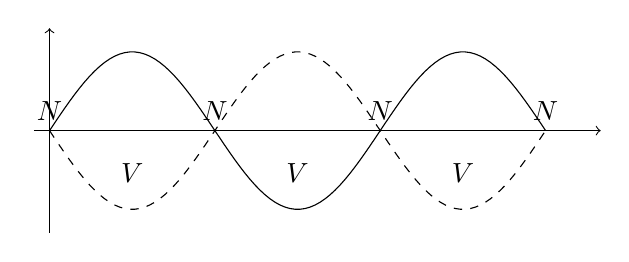
\begin{tikzpicture}[x=1cm,y=1cm]
\draw[->](-.2,0)--(7,0);\draw[->](0,-1.3)--(0,1.3);
\draw[domain=0:6.3,samples=100]plot(\x,{sin(180*\x/2.1)});
\draw[dashed,domain=0:6.3,samples=100]plot(\x,{-sin(180*\x/2.1)});
\foreach \x in {0,2.1,4.2,6.3}\node[above] at(\x,0){$N$};
\foreach \x in {1.05,3.15,5.25}\node[below]at(\x,-.3){$V$};
\end{tikzpicture}\end{center}
Ampiezza minima: $x=m\lambda/2$; massima: $x=(m+\tfrac12)\lambda/2$.
Supponiamo gli estremi della corda fissi: $\xi(0)=0$, $\xi(L)=0$; gli estremi sono nodi.
Per $m=1$, $L=\lambda/2$. In generale
\[L=m\lambda/2\iff\lambda=2L/m,\quad m\ge1.\]
Una lunghezza d'onda per ogni $m$:
\[f_i=\frac v{\lambda_i}=\frac{vi}{2L}.\]
$f_1$ ($m=1$) frequenza fondamentale (prima armonica); $f_2=2f_1$ seconda armonica; $f_n=nf_1$ $n$-esima armonica: frequenze armoniche.
% Pagina originale 14
\pagina{14}\section*{Orecchio umano}
Sensibilità da $20\ \mathrm{Hz}$ a $20\,000\ \mathrm{Hz}$. Sotto $20\ \mathrm{Hz}$: infrasuoni; sopra $20\ \mathrm{kHz}$: ultrasuoni.
La lunghezza d'onda varia fra $17.2\ \mathrm m$ e $1.72\ \mathrm{cm}$, ricordando $\lambda=v/f$.
Nel canale auricolare si producono onde stazionarie con
\[\lambda_m=\frac{4L}{2m+1},\qquad m=0,1,2,\ldots\]
\section*{Effetto Doppler}
Variazione apparente della frequenza di un'onda percepita da un osservatore in movimento rispetto alla sorgente.
Sorgente e osservatore fermi: $f'=f$; moto relativo: $f'\ne f$, dove $f'$ è la frequenza percepita e $f$ quella effettiva.
Caso 1: la sorgente si avvicina all'osservatore.
\[\lambda'=\lambda-v_{\rm sorg}T=\frac{v_{\rm onda}}f-\frac{v_{\rm sorg}}f=\frac{v_{\rm onda}-v_{\rm sorg}}f.\]
\[f'=\frac{v_{\rm onda}}{\lambda'}=f\frac{v_{\rm onda}}{v_{\rm onda}-v_{\rm sorg}}=\frac f{1-v_{\rm sorg}/v_{\rm onda}}>f.\]
% Pagina originale 15
\pagina{15}
Caso 2: la sorgente si allontana dall'osservatore.
\[\lambda'=\lambda+v_{\rm sorg}T=\frac{v_{\rm onda}+v_{\rm sorg}}f,\quad f'=\frac{v_{\rm onda}}{\lambda'}=f\frac{v_{\rm onda}}{v_{\rm onda}+v_{\rm sorg}}=\frac f{1+v_{\rm sorg}/v_{\rm onda}}<f.\]
Generalmente, sorgente in movimento:
\[f'=\frac f{1\pm v_{\rm sorg}/v_{\rm onda}},\]
$+$ allontanamento, $-$ avvicinamento.
Caso 3: l'osservatore si allontana dalla sorgente.
\[v_r=v_{\rm onda}-v_{\rm oss},\quad N=\frac{v_r\Delta t}\lambda\quad\text{numero di fronti incontrati},\]
\[f'=\frac N{\Delta t}=\frac{v_r}\lambda=\frac{v_{\rm onda}-v_{\rm oss}}{v_{\rm onda}}f=f\left(1-\frac{v_{\rm oss}}{v_{\rm onda}}\right)<f.\]
Caso 4: l'osservatore si avvicina alla sorgente.
\[v_r=v_{\rm onda}+v_{\rm oss},\quad N=\frac{v_r\Delta t}\lambda,\quad f'=\frac N{\Delta t}=\frac{v_r}\lambda=\frac{v_{\rm onda}+v_{\rm oss}}{v_{\rm onda}}f=f\left(1+\frac{v_{\rm oss}}{v_{\rm onda}}\right)>f.\]
% Pagina originale 16
\pagina{16}
Caso 5: sorgente e osservatore si muovono.
\[f'=f\frac{v_{\rm onda}\pm v_{\rm oss}}{v_{\rm onda}\mp v_{\rm sorg}}.\]
Segni $+/-$: avvicinamento; $-/+$: allontanamento.
Dove viene usato l'effetto Doppler? Autovelox, meteorologia, sirene antincendio.
\section*{Effetto Doppler per gli autovelox}
$f$ emessa; $f'$ riflessa; $f''$ misurata. $c$ velocità della luce, $v_m$ velocità della macchina.
\[f'=f\frac{c-v_m}c=f(1-v_m/c),\qquad f''=\frac{f'}{1+v_m/c}.\]
\[f''=f\frac{1-v_m/c}{1+v_m/c}=f\frac{(1-v_m/c)^2}{1-v_m^2/c^2}\simeq f(1-v_m/c)^2\simeq f(1-2v_m/c)=f-\frac{2v_m}\lambda,\]
poiché $(v_m/c)^2\ll1$.
\[\Delta f=|f''-f|=\left|-\frac{2v_m}\lambda\right|\implies v_m=\frac12\lambda\Delta f.\]
$\Delta f$ differenza fra frequenza emessa e misurata; negli appunti è poi usata come differenza con segno: $\Delta f>0$ avvicinamento, $\Delta f<0$ allontanamento.
Eco Doppler: effetto Doppler utilizzato nell'ecografia per visualizzare il movimento e la velocità degli oggetti in movimento (esempio: flusso del sangue).
% Pagina originale 17
\pagina{17}\section*{Onde elettromagnetiche}
Sfruttando le equazioni di Maxwell:
\begin{align*}
\vv\nabla\times\vv E&=-\partial_t\vv B,\\
\vv\nabla\times(\vv\nabla\times\vv E)&=-\vv\nabla\times\partial_t\vv B=-\partial_t(\vv\nabla\times\vv B),\\
&=-\mu_0\epsilon_0\partial_t^2\vv E,\\
\vv\nabla(\vv\nabla\cdot\vv E)-\nabla^2\vv E&=-\mu_0\epsilon_0\partial_t^2\vv E.
\end{align*}
Nel vuoto senza cariche $\vv\nabla\cdot\vv E=0$, dunque
\[\nabla^2\vv E=\mu_0\epsilon_0\partial_t^2\vv E\implies\partial_t^2\vv E=\frac1{\mu_0\epsilon_0}\nabla^2\vv E=c^2\nabla^2\vv E,\quad c=\frac1{\sqrt{\epsilon_0\mu_0}}.\]
Vale per ogni componente:
\[\partial_t^2E_x=c^2\nabla^2E_x,\quad\partial_t^2E_y=c^2\nabla^2E_y,\quad\partial_t^2E_z=c^2\nabla^2E_z.\]
Analogamente per $\vv B$ e ciascuna componente:
\begin{align*}
\vv\nabla\times\vv B&=\mu_0\epsilon_0\partial_t\vv E,\\
\vv\nabla\times(\vv\nabla\times\vv B)&=\mu_0\epsilon_0\partial_t(\vv\nabla\times\vv E)=\mu_0\epsilon_0\partial_t(-\partial_t\vv B),\\
\vv\nabla(\vv\nabla\cdot\vv B)-\nabla^2\vv B&=-\mu_0\epsilon_0\partial_t^2\vv B,\\
\partial_t^2\vv B&=\frac1{\mu_0\epsilon_0}\nabla^2\vv B=c^2\nabla^2\vv B.
\end{align*}
Le due equazioni hanno come soluzione:
% Pagina originale 18
\pagina{18}
\[\vv E=\vv E_0e^{i(\vv k\cdot\vv r-\omega t)},\qquad\vv B=\vv B_0e^{i(\vv k\cdot\vv r-\omega t)}.\]
\[\vv k=k_x\hat u_x+k_y\hat u_y+k_z\hat u_z,\qquad c=\omega/|\vv k|=\omega/k.\]
\[\partial_t^2E_x=\frac1{\mu_0\epsilon_0}(\partial_x^2E_x+\partial_y^2E_x+\partial_z^2E_x),\qquad E_x=E_{0x}e^{i(k_xx+k_yy+k_zz-\omega t)}.\]
Osserviamo $\vv E=E_x\hat u_x+E_y\hat u_y+E_z\hat u_z$:
\[\vv\nabla\cdot\vv E=\partial_xE_x+\partial_yE_y+\partial_zE_z=i(k_xE_x+k_yE_y+k_zE_z)=0\implies\vv k\cdot\vv E=0.\]
Analogamente $\vv k\cdot\vv B=0$.
Dalle componenti di $\vv\nabla\times\vv E=-\partial_t\vv B$:
\[ik_yE_z-ik_zE_y=i\omega B_x,\quad ik_zE_x-ik_xE_z=i\omega B_y,\quad ik_xE_y-ik_yE_x=i\omega B_z.\]
\[\vv k\times\vv E=\omega\vv B\implies kE=\omega B\implies E=(\omega/k)B=cB.\]
$\vv E\cdot\vv B=0$: perpendicolari; $\vv E\perp\vv B$, entrambe perpendicolari alla propagazione.
% Pagina originale 19
\pagina{19}
$\vv E\times\vv B$ indica la direzione di propagazione.
\[\vv E\times\vv B=\frac1\omega\vv E\times(\vv k\times\vv E)=\frac1\omega[\vv k(\vv E\cdot\vv E)-\vv E(\vv E\cdot\vv k)]=\frac1\omega\vv kE^2=\frac{E^2}c\hat u_k=EB\hat u_k.\]
Proprietà onde EM:
\begin{enumerate}\item $\vv E$ e $\vv B$ si propagano alla velocità della luce.\item $B=E/c\iff E=Bc$.\item $\vv E\perp\vv B$.\item $\vv E\times\vv B$ fornisce il verso di propagazione $\hat u_k$.\end{enumerate}
Caso di propagazione semplice in un solo asse ($x$):
\[\vv E=E_0e^{i(kx-\omega t)}\hat u_y,\qquad\vv B=B_0e^{i(kx-\omega t)}\hat u_z.\]
\section*{Onde di propagazione generale (onde piane)}
Propagazione nell'asse $x$, campo elettrico e magnetico nel piano $yz$:
\[\vv E=E_{0y}e^{i(kx-\omega t)}\hat u_y+E_{0z}e^{i(kx-\omega t)}\hat u_z,\]
\[\vv B=B_{0y}e^{i(kx-\omega t)}\hat u_y+B_{0z}e^{i(kx-\omega t)}\hat u_z.\]
% Pagina originale 20
\pagina{20}
Ricordando $\vv k\times\vv E=\omega\vv B$ e $\vv k=k\hat u_x$:
\[-kE_z=\omega B_y,\quad kE_y=\omega B_z,\quad B_y=-E_z/c,\quad B_z=E_y/c,\quad E_z=-B_yc,\quad E_y=B_zc.\]
\[\vv B=\hat u_zE_y/c-\hat u_yE_z/c,\quad\vv E=\hat u_yB_zc-\hat u_zB_yc,\]
\[\vv E=(0,B_zc,-B_yc),\quad\vv B=(0,-E_z/c,E_y/c)=(0,B_y,B_z).\]
\[\vv E\cdot\vv B=B_yB_zc-B_zB_yc=0.\]
\[\vv E\times\vv B=\begin{vmatrix}\hat u_x&\hat u_y&\hat u_z\\0&B_zc&-B_yc\\0&B_y&B_z\end{vmatrix}=c(B_y^2+B_z^2)\hat u_x=cB^2\hat u_x=EB\hat u_x=\frac{E^2}c\hat u_x.\]
\section*{Onde nei dielettrici}
L'unica equazione di Maxwell che cambia è $\vv\nabla\times\vv B=\mu\epsilon\partial_t\vv E$, con $\mu\epsilon=1/v^2$.
\[v=\frac1{\sqrt{\mu\epsilon}}=\frac1{\sqrt{\epsilon_0\mu_0}}\frac1{\sqrt{\mu_r\epsilon_r}}=\frac c{\sqrt{\mu_r\epsilon_r}}<c.\]
Nella maggior parte dei mezzi ordinari $\mu_r=1$, quindi $v=c/\sqrt{\epsilon_r}=c/n$; $n$ indice di rifrazione del mezzo.
\[Z_0=\sqrt{\mu_0/\epsilon_0}=377\ \Omega\quad\text{impedenza nel vuoto},\qquad Z=Z_0/n\quad\text{impedenza nel mezzo}.\]
% Pagina originale 21
\pagina{21}\section*{Vettore di Poynting}
\[\vec S=\frac1{\mu_0}\vec E\times\vec B=\frac{EB}{\mu_0}\hat u_k,\qquad \vec S\parallel\hat u_k\parallel\vec k,\qquad |\vec S|=\frac{EB}{\mu_0}.\]
Il modulo rappresenta l'energia elettromagnetica che passa in un secondo per ogni metro quadrato. Le onde EM trasportano energia e non solo: esse riescono a trasferire quantità di moto esercitando una pressione di ``radiazione''.
\[p_{\rm rad}=\frac Ic\quad\text{(onda completamente assorbita)},\qquad p_{\rm rad}=\frac{2I}c\quad\text{(onda totalmente riflessa)}.\]
Se l'onda è in parte riflessa e in parte assorbita,
\[p_{\rm rad}\in(I/c,2I/c),\qquad p_{\rm rad}=\frac Ic(1+r_R),\]
con $r_R$ coefficiente, percentuale di riflessione [simbolo manoscritto poco chiaro]. Se l'onda forma un angolo $\theta>0$ con la normale alla superficie $\Sigma$:
\[p_{\rm rad}=\frac Ic\cos^2\theta\quad\text{(assorbimento)},\qquad p_{\rm rad}=\frac{2I}c\cos^2\theta\quad\text{(riflessione)}.\]
Ricordiamo che $I=P/\Sigma$ e $I=\tfrac12\epsilon_0cE^2$, dove $\epsilon_0=8.85\cdot10^{-12}\,\mathrm{F/m}$ è la permittività del vuoto.
% Pagina originale 22
\pagina{22}\section*{Tipi di onde EM}
\begin{center}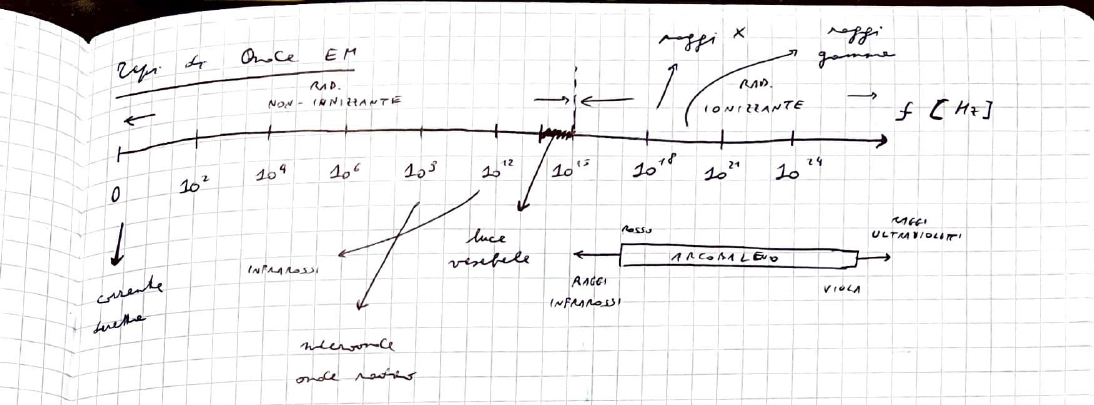
\includegraphics[width=.95\linewidth]{ottica_tex_assets/b21_p22_spectrum.png}\end{center}
\begin{center}\begin{tabular}{ll}Rosso&$780$--$622$ nm\\Arancione&$622$--$597$ nm\\Giallo&$597$--$577$ nm\\Verde&$577$--$492$ nm\\Azzurro&$492$--$455$ nm\\Violetto&$455$--$380$ nm\end{tabular}\end{center}
I colori che vediamo sono la sovrapposizione delle onde EM riflesse dal materiale dell'oggetto. Il nero assorbe tutto. Il bianco riflette tutto.
\section*{Produzione di onde EM}
L'oscillazione di due cariche di segno opposto produce una perturbazione delle linee di campo che si propaga nello spazio. La coppia di cariche elettriche (detta dipolo oscillante) oscillanti è chiamata ``antenna''.
\begin{center}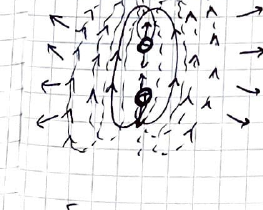
\includegraphics[width=.23\linewidth]{ottica_tex_assets/b21_p22_dipole.png}\end{center}
Si produce un campo elettrico $E$ per presenza di cariche elettriche; si produce un campo magnetico per presenza di cariche elettriche in movimento. Per produrre (e ricevere) un'onda EM si utilizza un circuito RLC.
% Pagina originale 23
\pagina{23}
\begin{center}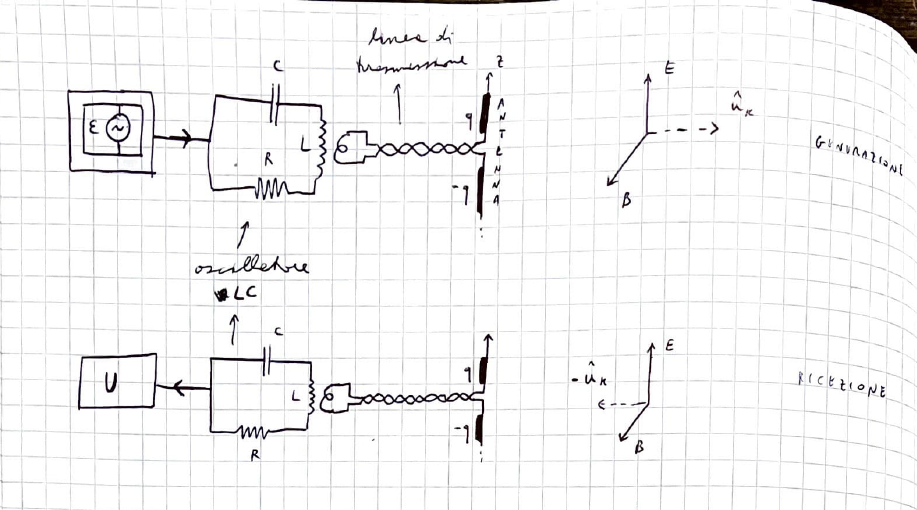
\includegraphics[width=.9\linewidth]{ottica_tex_assets/b21_p23_circuit.png}\end{center}
Il campo elettrico generato dall'antenna è un'onda sferica:
\[E=E_\theta=\frac{p_0\sin\theta}{4\pi\epsilon_0c^2}\frac{\omega^2}{r}\sin(kr-\omega t),\qquad r\gg\lambda\gg\text{dimensione del dipolo}.\]
\[E\propto\frac1r\quad\text{come quasi sempre per le onde sferiche},\qquad E=0\text{ per }\theta=k\pi,\quad k=0,1,\ldots\]
Il campo non c'è lungo l'asse del dipolo. L'intensità è calcolabile con la formula $I=\tfrac12\epsilon_0cE_0^2$. La potenza vale
\[P=\frac{8\pi}{3}I_0,\qquad P=\int_\Sigma I(r,\theta)\,d\Sigma.\]
\section*{Polarizzazione delle onde EM}
\begin{center}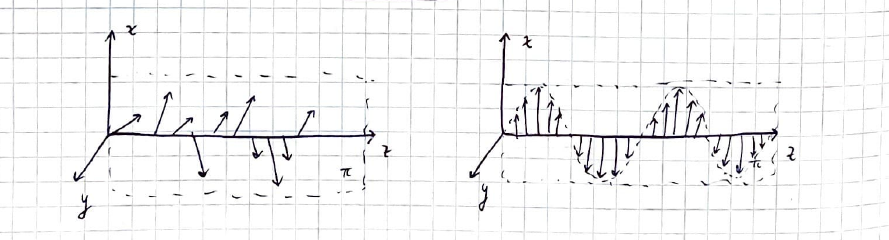
\includegraphics[width=.85\linewidth]{ottica_tex_assets/b21_p23_polarization.png}\end{center}
Onda piana non polarizzata; onda piana polarizzata rettilineamente.
% Pagina originale 24
\pagina{24}\section*{Polarizzazione rettilinea}
\[\hat u_p=\hat u_E\quad\text{direzione di polarizzazione}.\]
Il piano contenente $\vec E$ e $\vec k$ è il piano di propagazione.
\begin{center}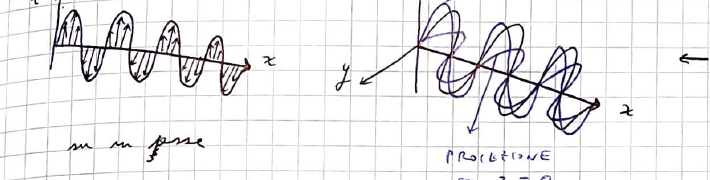
\includegraphics[width=.85\linewidth]{ottica_tex_assets/b21_p24_wave.png}\end{center}
In generale
\[E_y(x,t)=E_{0y}\cos(kx-\omega t+\delta),\qquad E_z(x,t)=E_{0z}\cos(kx-\omega t).\]
Se $\delta=k\pi$ si ha una polarizzazione rettilinea. Se $\delta=\tfrac{2k+1}{2}\pi$ si ha una polarizzazione circolare.
\begin{center}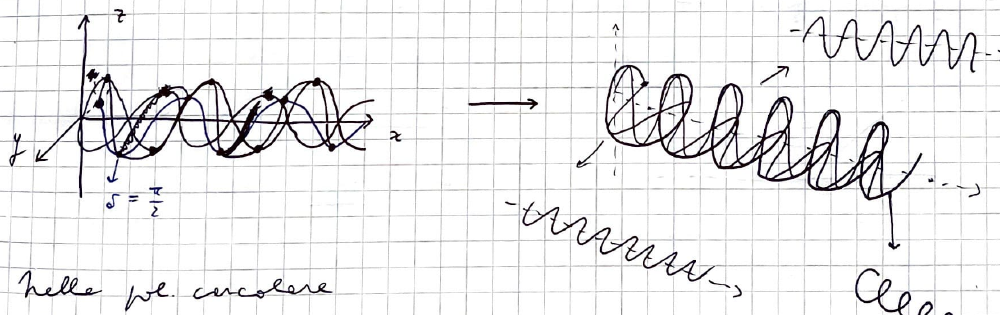
\includegraphics[width=.9\linewidth]{ottica_tex_assets/b21_p24_circular.png}\end{center}
Nella polarizzazione circolare
\[\frac{E_y^2}{E_{0y}^2}+\frac{E_z^2}{E_{0z}^2}=1.\]
Nelle onde non polarizzate $\delta$ è variabile.
\section*{Lamine polarizzatrici}
Trasmettono solo la componente lungo la direzione dell'asse ottico.
% Pagina originale 25
\pagina{25}
\begin{center}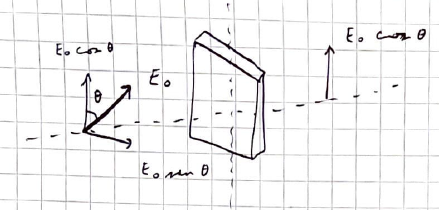
\includegraphics[width=.5\linewidth]{ottica_tex_assets/b21_p25_malus.png}\end{center}
Viene trasmessa solo la componente parallela all'asse polarizzatore, $E_0\cos\theta$; la componente ortogonale è $E_0\sin\theta$.
\[I'=I_0\cos^2\theta\qquad\text{(legge di Malus)}.\]
Cambia l'intensità trasmessa. $I'=I_0/2$ nel caso di radiazione non polarizzata. Su questo effetto si basa il 3D (occhiali 3D).
\section*{Riflessione e rifrazione}
Riflessione: avviene all'interno dello stesso materiale ($n_1=n_2$, indice di rifrazione).
\[\theta_1=\theta_2\quad\text{(prima legge)}.\]
Il raggio incidente $i$, il riflesso $r$ e la normale $o$ sono complanari (seconda legge).
Rifrazione: avviene quando l'onda cambia mezzo di trasmissione ($n_1\ne n_2$).
\[n_1\sin\theta_1=n_2\sin\theta_2\quad\text{(prima legge, legge di Snell)}.\]
Il raggio incidente $i$, il trasmesso (rifratto) $t$ e la normale $o$ sono complanari (seconda legge).
\[n=\frac cv,\qquad n\ge1\quad\forall\text{ materiale}.\]
\begin{center}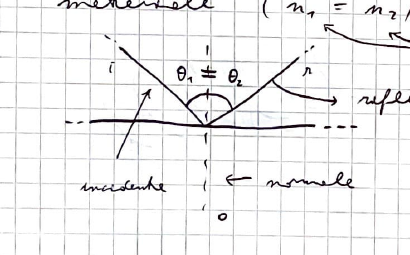
\includegraphics[width=.46\linewidth]{ottica_tex_assets/b21_p25_reflection.png}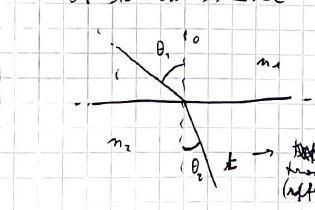
\includegraphics[width=.46\linewidth]{ottica_tex_assets/b21_p25_refraction.png}\end{center}
% Pagina originale 26
\pagina{26}
\begin{center}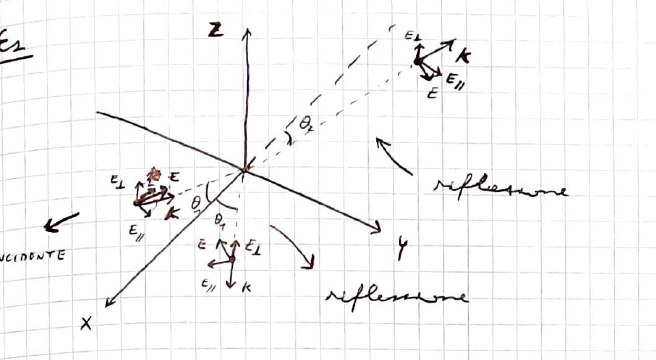
\includegraphics[width=.62\linewidth]{ottica_tex_assets/b21_p26_geometry.png}\end{center}
\begin{align*}
k_{i,y}=k_{r,y}&\implies k_i\sin\alpha=k_r\sin\beta\implies\frac\omega c n_1\sin\alpha=\frac\omega c n_1\sin\beta\implies\alpha=\beta,\\
k_{i,y}=k_{t,y}&\implies k_i\sin\alpha=k_t\sin\beta\implies\frac\omega c n_1\sin\alpha=\frac\omega c n_2\sin\beta\implies n_1\sin\alpha=n_2\sin\beta.
\end{align*}
Leggi di Snell per riflessione e rifrazione.
\section*{Condizioni di raccordo}
\begin{align*}
E_{1\parallel}=E_{2\parallel}&\implies D_{1\parallel}/\epsilon_1=D_{2\parallel}/\epsilon_2,\\
D_{1\perp}=D_{2\perp}&\implies\epsilon_1E_{1\perp}=\epsilon_2E_{2\perp},\\
H_{1\parallel}=H_{2\parallel}&\implies B_{1\parallel}/\mu_1=B_{2\parallel}/\mu_2,\\
B_{1\perp}=B_{2\perp}&\implies\mu_1H_{1\perp}=\mu_2H_{2\perp}.
\end{align*}
Ricordiamo $D=\epsilon E$, $B=\mu H$. Possiamo esaminare due tipi di polarizzazione: $\sigma$ ($s$), ortogonale al piano di incidenza; $\pi$ ($p$), parallela al piano di incidenza. Ora troviamo le formule di raccordo di $E$ e $B$ nel passaggio da un materiale con indice di rifrazione $n_1$ a uno con indice $n_2\ne n_1$.
% Pagina originale 27
\pagina{27}\section*{Polarizzazione $\sigma$ rispetto a $E$}
\begin{center}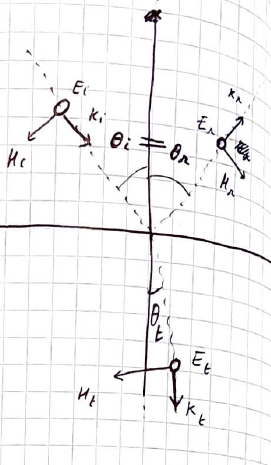
\includegraphics[width=.38\linewidth]{ottica_tex_assets/b21_p27_geometry.png}\end{center}
\begin{align*}
E_{1\parallel}=E_{2\parallel}&\implies E_i+E_r=E_t,\\
H_{1\parallel}=H_{2\parallel}&\implies H_i'+H_r'=H_t',\\
-H_i\cos\theta_i+H_r\cos\theta_r&=-H_t\cos\theta_t.
\end{align*}
Poiché $\theta_i=\theta_r$, $H_r-H_i=-\chi H_t$, con $\chi=\cos\theta_t/\cos\theta_i$.
\[H=\frac B\mu=\frac E{\mu v}=\frac{E\sqrt{\epsilon\mu}}\mu=E\sqrt{\frac\epsilon\mu}=E\sqrt{\frac{\epsilon_0\epsilon_r}{\mu_0\mu_r}}=E\sqrt{\frac{\epsilon_0}{\mu_0}}\sqrt{\epsilon_r}=E\frac n{Z_0}.\]
\[H_r-H_i=-\chi H_t\implies\frac{E_r}{Z_0}n_1-\frac{E_i}{Z_0}n_1=-\chi\frac{E_t}{Z_0}n_2\implies E_r-E_i=-\chi E_t\frac{n_2}{n_1}.\]
Ponendo $\eta=n_2/n_1$:
\[\begin{cases}E_i+E_r=E_t\\E_i-E_r=\chi\eta E_t\end{cases}\implies\begin{cases}E_r=\dfrac{1-\eta\chi}{1+\eta\chi}E_i\\E_t=\dfrac2{1+\eta\chi}E_i.\end{cases}\]
\[r_\sigma=\frac{E_r}{E_i}=\frac{1-\eta\chi}{1+\eta\chi},\qquad t_\sigma=\frac{E_t}{E_i}=\frac2{1+\eta\chi}.\]
$r_\sigma$ è il coefficiente di riflessione per polarizzazione $\sigma$; $t_\sigma$ è il coefficiente di trasmissione per polarizzazione $\sigma$.
% Pagina originale 28
\pagina{28}\section*{Polarizzazione $\pi$ rispetto a $E$}
\begin{center}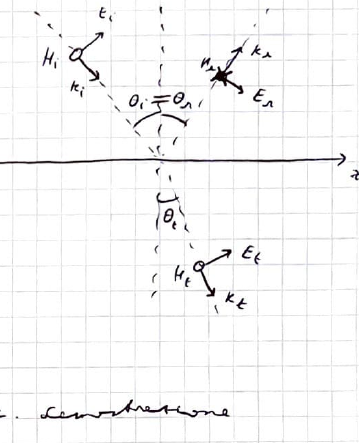
\includegraphics[width=.38\linewidth]{ottica_tex_assets/b21_p28_geometry.png}\end{center}
\begin{align*}
H_{1\parallel}=H_{2\parallel}&\implies H_i-H_r=H_t,\\
E_{1\parallel}=E_{2\parallel}&\implies E_i\cos\theta_i+E_r\cos\theta_r=E_t\cos\theta_t\implies E_i+E_r=\chi E_t.
\end{align*}
$H=En/Z_0$, come visto nella precedente dimostrazione:
\[E_i\frac{n_1}{Z_0}-E_r\frac{n_1}{Z_0}=E_t\frac{n_2}{Z_0}\implies E_i-E_r=\eta E_t.\]
\[\begin{cases}E_i+E_r=\chi E_t\\E_i-E_r=\eta E_t\end{cases}\implies\begin{cases}E_r=\dfrac{\chi-\eta}{\chi+\eta}E_i\\E_t=\dfrac2{\chi+\eta}E_i.\end{cases}\]
\[r_\pi=\frac{E_r}{E_i}=\frac{\chi-\eta}{\chi+\eta},\qquad t_\pi=\frac{E_t}{E_i}=\frac2{\chi+\eta},\qquad\eta=\frac{n_2}{n_1},\quad\chi=\frac{\cos\theta_t}{\cos\theta_i}.\]
$r_\pi$ è il coefficiente di riflessione per polarizzazione $\pi$; $t_\pi$ è il coefficiente di trasmissione per polarizzazione $\pi$.
\section*{Angolo limite}
Esiste $\theta_0$, detto ``angolo limite'', con
\[\theta_0=\arcsin\frac{n_2}{n_1},\qquad n_1>n_2.\]
Se si forma un angolo $\theta>\theta_0$ non ci sarà trasmissione ma solo riflessione. $n_1$: sorgente; $n_2$: destinazione. Se $n_1<n_2$ non esiste un angolo limite; ogni $\theta\in[0,\pi/2)$ è disponibile per la rifrazione.
% Pagina originale 29
\pagina{29}
$t_\sigma$ e $t_\pi$ sono sempre positivi. $r_\sigma$ e $r_\pi$ sono sempre positivi quando $n_1>n_2$, sempre negativi quando $n_1<n_2$ [affermazione trascritta dall'originale]. $r$ e $t$ sono chiamati coefficienti di Fresnel.
\section*{Energia}
\[W=I\Sigma_0\cos\theta,\qquad I=\tfrac12\epsilon v E^2.\]
\begin{align*}
W_i&=\frac12\frac c{\sqrt{\epsilon_{r1}}}\epsilon_{r1}\epsilon_0|E_i|^2\Sigma_0\cos\theta_i,\\
W_r&=\frac12\frac c{\sqrt{\epsilon_{r1}}}\epsilon_{r1}\epsilon_0|E_r|^2\Sigma_0\cos\theta_i,\\
W_t&=\frac12\frac c{\sqrt{\epsilon_{r2}}}\epsilon_{r2}\epsilon_0|E_t|^2\Sigma_0\cos\theta_t.
\end{align*}
\[R_\sigma=\frac{W_r}{W_i}=\frac{|E_r|^2}{|E_i|^2}=r_\sigma^2,\qquad T_\sigma=\frac{W_t}{W_i}=\frac{|E_t|^2}{|E_i|^2}\sqrt{\frac{\epsilon_{r2}}{\epsilon_{r1}}}\chi=\eta\chi t_\sigma^2.\]
\[R_\pi=r_\pi^2,\qquad T_\pi=\eta\chi t_\pi^2,\qquad\sqrt{\epsilon_{r2}/\epsilon_{r1}}=n_2/n_1=\eta.\]
\begin{align*}
R_\sigma+T_\sigma=1&\iff r_\sigma^2+\eta\chi t_\sigma^2=1\\
&\iff\frac{(1-\eta\chi)^2}{(1+\eta\chi)^2}+\eta\chi\frac4{(1+\eta\chi)^2}=1\\
&\iff(1-\eta\chi)^2+4\eta\chi=(1+\eta\chi)^2\\
&\iff-2\eta\chi+4\eta\chi=2\eta\chi.
\end{align*}
\section*{Caso di incidenza normale}
Non è più definibile il piano di incidenza $\pi$.
\[r_\sigma=\frac{1-\eta\chi}{1+\eta\chi},\quad t_\sigma=\frac2{1+\eta\chi},\qquad r_\pi=\frac{\chi-\eta}{\chi+\eta},\quad t_\pi=\frac2{\chi+\eta},\quad\chi=1.\]
% Pagina originale 30
\pagina{30}
Poiché $\theta_i=\theta_r=\theta_t=0$, $\chi=1$:
\[r_\sigma=r_\pi=\frac{1-\eta}{1+\eta},\qquad t_\sigma=t_\pi=\frac2{1+\eta}.\]
$\sigma$ e $\pi$ coincidono. Se $n_1<n_2$ (aria $\to$ vetro), $r_\sigma<0$, $t_\sigma>0$. Se $n_1>n_2$ (vetro $\to$ aria), $r_\sigma>0$, $t_\sigma>0$.
\begin{center}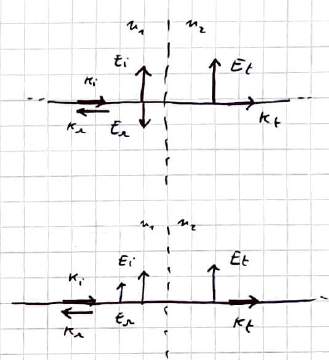
\includegraphics[width=.45\linewidth]{ottica_tex_assets/b21_p30_signs.png}\end{center}
\section*{Angolo di Brewster}
\[\exists\theta_B\in(0,\pi/2):R_\pi=0,\qquad R_\pi=r_\pi^2=\frac{\tan^2(\theta_i-\theta_t)}{\tan^2(\theta_i+\theta_t)}.\]
\begin{center}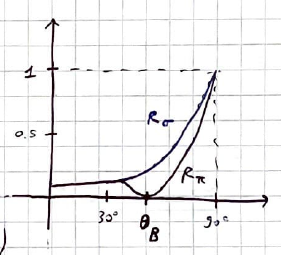
\includegraphics[width=.45\linewidth]{ottica_tex_assets/b21_p30_graph.png}\end{center}
Se $\theta_i+\theta_t=\pi/2$, allora $R_\pi=0\implies r_\pi^2=0\implies r_\pi=0\implies E_r=0$: non c'è riflessione. Calcoliamo $\theta_B$:
\[\theta_B+\theta_t=\pi/2,\qquad\frac{n_2}{n_1}=\frac{\sin\theta_i}{\sin\theta_t}=\frac{\sin\theta_B}{\sin(\pi/2-\theta_B)}=\frac{\sin\theta_B}{\cos\theta_B}=\tan\theta_B.\]
\[\tan\theta_B=\eta\implies\theta_B=\arctan\eta.\]
% Pagina originale 31
\pagina{31}
L'angolo di Brewster e l'angolo critico/limite,
\[\theta_B=\arctan\eta,\qquad\theta_0=\arcsin\eta,\]
sono angoli particolari, dove c'è totale rifrazione o totale riflessione (cioè $r_\pi(\theta_B)=0$ e $t_\pi(\theta_0)=0$). Con $\theta_i=\theta_B$ non c'è riflessione. Con $\theta_i\ge\theta_0$ non c'è rifrazione.
\section*{Passaggio nei materiali}
Le caratteristiche delle onde che cambiano da un materiale a un altro sono:
\begin{align*}
v&=\frac c{\sqrt{\epsilon_r}}=\frac cn,&v_0&=c,&\frac v{v_0}&=\frac1n,\\
k&=\frac\omega v=\frac\omega c n,&k_0&=\frac\omega c,&\frac k{k_0}&=n,\\
\lambda&=\frac{2\pi}k=\frac{2\pi c}{\omega n},&\lambda_0&=\frac{2\pi c}\omega,&\frac\lambda{\lambda_0}&=\frac1n.
\end{align*}
$f$ e $\omega=2\pi f$ rimangono invariati:
\[f=\frac v\lambda=\frac v\lambda\frac{v_0}v\frac\lambda{\lambda_0}=\frac v\lambda\frac1n n=f_0=f.\]
\[n=\frac cv=\frac k{k_0}=\frac{\lambda_0}\lambda=\sqrt{\epsilon_r}.\]
% Pagina originale 32
\pagina{32}\section*{Principio di Fermat}
Cammino geometrico: $L_g=\overline{PQ}+\overline{QP'}$. Cammino ottico: $L_n=n_1\overline{PQ}+n_2\overline{QP'}$.
\subsection*{Riflessione}
\begin{center}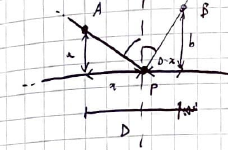
\includegraphics[width=.4\linewidth]{ottica_tex_assets/b21_p32_reflection.png}\end{center}
\[L=\sqrt{a^2+x^2}+\sqrt{b^2+(D-x)^2},\qquad t=L/c.\]
\begin{align*}
\frac{\partial t}{\partial x}=0&\implies\frac1c\frac{dL}{dx}=\frac1{2c}(a^2+x^2)^{-1/2}2x-\frac1{2c}[b^2+(D-x)^2]^{-1/2}2(D-x)=0\\
&\implies\frac x{\sqrt{a^2+x^2}}=\frac{D-x}{\sqrt{b^2+(D-x)^2}}\\
&\implies\sin\theta_i=\sin\theta_r\implies\boxed{\theta_i=\theta_r}.
\end{align*}
\subsection*{Rifrazione}
\begin{center}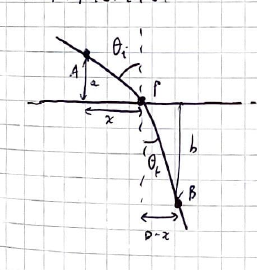
\includegraphics[width=.4\linewidth]{ottica_tex_assets/b21_p32_refraction.png}\end{center}
\[L=n_1\underbrace{\sqrt{a^2+x^2}}_{L_1}+n_2\underbrace{\sqrt{b^2+(D-x)^2}}_{L_2},\qquad t=L/c=n_1L_1/c+n_2L_2/c=t_{AP}+t_{PB}.\]
\[\frac{\partial t}{\partial x}=0\implies n_1\frac x{\sqrt{a^2+x^2}}=n_2\frac{D-x}{\sqrt{b^2+(D-x)^2}}\implies\boxed{n_1\sin\theta_i=n_2\sin\theta_t}\quad\text{legge di Snell}.\]
% Pagina originale 33
\pagina{33}\section*{Attraversamento di lamina piana}
\begin{center}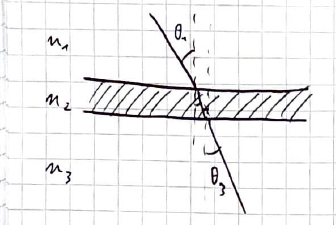
\includegraphics[width=.38\linewidth]{ottica_tex_assets/b21_p33_slab.png}\end{center}
Se $n_1=n_3$ (stesso materiale), allora $\theta_1=\theta_3$. Dimostrazione:
\[n_1\sin\theta_1=n_2\sin\theta_2=n_3\sin\theta_3\implies n_1\sin\theta_1=n_1\sin\theta_3\implies\theta_1=\theta_3.\]
L'angolo con il quale è entrato il raggio sarà lo stesso con il quale esce.
\section*{Effetti visivi della rifrazione}
\begin{center}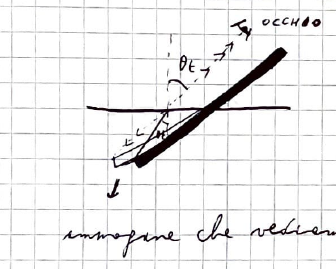
\includegraphics[width=.4\linewidth]{ottica_tex_assets/b21_p33_apparent.png}\end{center}
L'immagine che vediamo è più vicina (apparente) e meno obliqua, come in figura.
\section*{Angolo di deviazione}
Consideriamo un prisma. In questo caso l'attraversamento di un oggetto porta a una deviazione dell'onda perché cambiano il primo e il secondo normale ($o_1\not\parallel o_2$).
\begin{center}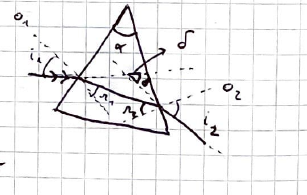
\includegraphics[width=.42\linewidth]{ottica_tex_assets/b21_p33_prism.png}\end{center}
\[\delta=(i_1-r_1)+(i_2-r_2),\qquad\alpha=\pi-[(\pi/2-r_1)+(\pi/2-r_2)]=r_1+r_2\implies\delta=i_1+i_2-\alpha.\]
% Pagina originale 34
\pagina{34}
\[\begin{cases}\delta=i_1+i_2-\alpha\\\alpha=r_1+r_2\\\sin i_1=n\sin r_1\\n\sin r_2=\sin i_2\end{cases}\implies\begin{cases}\dfrac{d\delta}{di_1}=1+\dfrac{di_2}{di_1}\\dr_1+dr_2=0\quad(\alpha\text{ costante})\\\cos i_1\,di_1=n\cos r_1\,dr_1\\n\cos r_2\,dr_2=\cos i_2\,di_2.\end{cases}\]
Per trovare $\delta_{\min}$ annulliamo $d\delta/di_1$, quindi $di_2/di_1=-1$ [nel manoscritto il rapporto appare invertito, equivalente qui]. Con alcuni passaggi geometrici arriviamo a
\[\sin^2i_1=\sin^2i_2\implies i_1=i_2=i,\qquad r_1=r_2=r.\]
\[\begin{cases}\delta_{\min}=2i-\alpha\\\alpha=2r\end{cases}\qquad n=\frac{\sin i_1}{\sin r_1}=\frac{\sin i}{\sin r}=\frac{\sin\dfrac{\alpha+\delta_{\min}}2}{\sin\dfrac\alpha2}.\]
\section*{Ottica geometrica}
Oggetto: corpo che emette luce propria o diffonde luce di un altro corpo. Strumento ottico: apparato che riflette o rifrange la luce emessa da un oggetto. Immagine: luce emessa dall'oggetto trasformata da uno strumento ottico e raccolta su uno schermo. Ottica geometrica: materia che studia la formazione di immagini mediante strumenti ottici.
Nell'ottica geometrica non entra in gioco la natura ondulatoria della luce poiché la lunghezza d'onda è di molto inferiore alle superfici degli strumenti ottici.
% Pagina originale 35
\pagina{35}\section*{Elemento ottico}
\begin{center}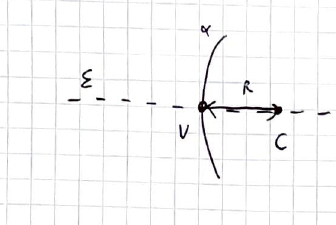
\includegraphics[width=.4\linewidth]{ottica_tex_assets/b21_p35_element.png}\end{center}
$C$: centro; $R$: raggio di curvatura; $V$: intersezione fra asse e superficie, vertice.
Una superficie che presenta solo riflessione è detta superficie catottrica (specchio). Una superficie che presenta rifrazione è detta superficie diottrica (diottro). Una lente è l'insieme di due diottri opportunamente disposti. Un elemento è stigmatico se trasforma un punto oggetto in un unico punto immagine.
\section*{Specchio concavo}
\begin{center}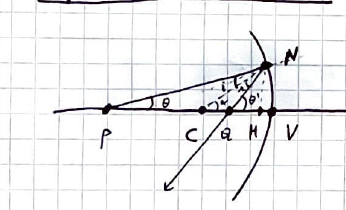
\includegraphics[width=.43\linewidth]{ottica_tex_assets/b21_p35_mirror.png}\end{center}
\[\theta+i=\alpha,\qquad\theta'=\alpha+r\implies\theta+\theta'=2\alpha,\qquad i=r=\widehat{CNQ}.\]
\begin{align*}y&=NV\simeq NH\quad\text{distanza trasversale},\\p&=PV\simeq PH\quad\text{distanza dell'oggetto da }V,\\q&=QV\simeq QH\quad\text{distanza dell'immagine da }V.\end{align*}
In ottica gaussiana $HV\simeq0$, quindi $\tan\theta\simeq\sin\theta\simeq\theta$.

% Pagina originale 36
\pagina{36}
\[
\tan\theta=\frac{NH}{PH},\qquad
\tan\theta'=\frac{NH}{QH},\qquad
\tan\alpha=\frac{NH}{CH}.
\]
\[
\theta\simeq\tan\theta\simeq\frac yp,\qquad
\theta'\simeq\tan\theta\simeq\frac yq,\qquad
\alpha\simeq\tan\alpha\simeq\frac yR.
\]
\[
\theta+\theta'=2\alpha\quad\Longrightarrow\quad
\frac yp+\frac yq=\frac{2y}{R}
\quad\Longrightarrow\quad \frac1p+\frac1q=\frac2R.
\]
\subsubsection*{Specchio concavo: fuoco}
\begin{center}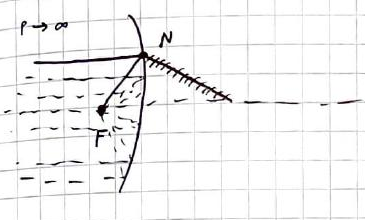
\includegraphics[width=.45\linewidth]{ottica_tex_assets/b36_p36_1.png}\end{center}
\[
P\longrightarrow\infty\quad\Longrightarrow\quad
p\longrightarrow\infty\quad\Longrightarrow\quad\frac1p\longrightarrow0,
\qquad
\frac1p+\underbrace{\frac1q}_{1/f}=\frac2R
\quad\Longrightarrow\quad f=\frac R2.
\]
Per il principio di invertibilità del raggio luminoso, qualunque raggio che parte dal fuoco, dopo aver colpito lo specchio, viene riflesso parallelamente all'asse. Cambiando verso di percorrenza il percorso rimane invariato, solo percorso nel verso opposto ma identico:
\[
p=f\quad\Longrightarrow\quad q\longrightarrow\infty.
\]
Se $P\in(F,V)$ i raggi divergeranno.
\begin{center}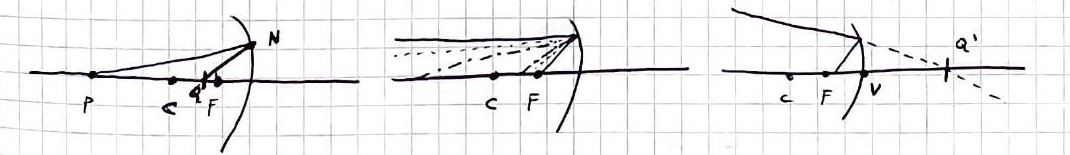
\includegraphics[width=\linewidth]{ottica_tex_assets/b36_p36_2.png}\end{center}
È il prolungamento del raggio ad intersecarsi con le superficie. Si parla in questo caso di \emph{immagine virtuale}.
\[
\frac1p-\frac1q=\frac2R.
\]
% Nella seconda approssimazione la scansione scrive tan(theta) anziché tan(theta').
% Pagina originale 37
\pagina{37}
\subsubsection*{Specchio convesso}
\begin{center}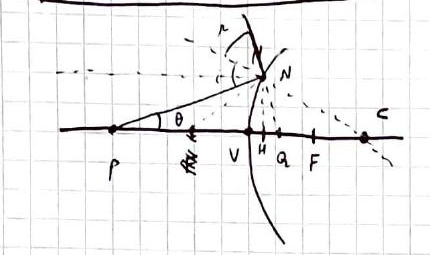
\includegraphics[width=.5\linewidth]{ottica_tex_assets/b36_p37_1.png}\end{center}
\[
i=\theta+\alpha,\qquad \theta'=r+\alpha
\quad\Longrightarrow\quad\theta'-\theta=2\alpha.
\]
\[
\tan\theta=\frac{NH}{PH},\qquad
\tan\theta'=\frac{NH}{QH},\qquad
\tan\alpha=\frac{NH}{CH},\qquad
 y=NH,\quad p=PH,\quad q=QH.
\]
\[
\theta\simeq\tan\theta,\qquad\theta'\simeq\tan\theta',\qquad
\alpha\simeq\tan\alpha.
\]
\[
\frac yq-\frac yp=\frac{2y}{R}
\quad\Longrightarrow\quad\frac1q-\frac1p=\frac2R
\qquad\left(\frac1p-\frac1q=-\frac2R\right).
\]
\[
p\longrightarrow\infty\quad\Longrightarrow\quad f=\frac R2.
\]
Nello specchio convesso l'immagine è sempre virtuale.
\subsubsection*{Convenzione dei segni}
\begin{center}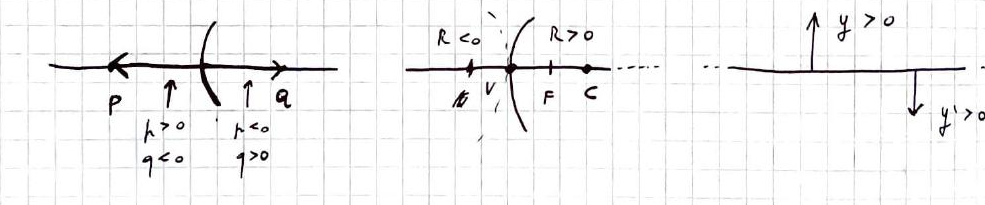
\includegraphics[width=\linewidth]{ottica_tex_assets/b36_p37_2.png}\end{center}
A sinistra del vertice: $p>0$, $q<0$; a destra: $p<0$, $q>0$.
$R<0$ a sinistra, $R>0$ a destra. Sopra l'asse $y>0$; sotto l'asse nel disegno è indicato $y'>0$.
% Il disegno originale riporta y'>0 sotto l'asse; etichetta conservata.
\[
\frac1{|p|}+\frac1{|q|}=\frac2{|R|},\qquad
\frac1{|p|}-\frac1{|q|}=\frac2{|R|},\qquad
\frac1{|p|}-\frac1{|q|}=-\frac2{|R|}.
\]
\[
\boxed{\frac1p-\frac1q=-\frac2R}.
\]
\begin{center}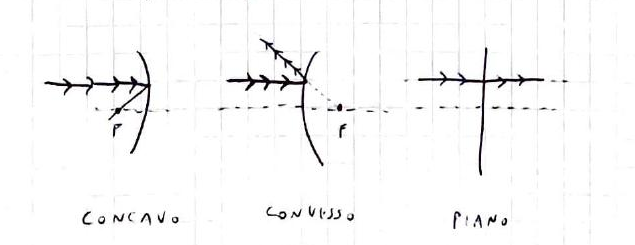
\includegraphics[width=.85\linewidth]{ottica_tex_assets/b36_p37_3.png}\end{center}
Specchio concavo, convesso, piano.
% Pagina originale 38
\pagina{38}
\subsubsection*{Costruzione dell'immagine}
\begin{center}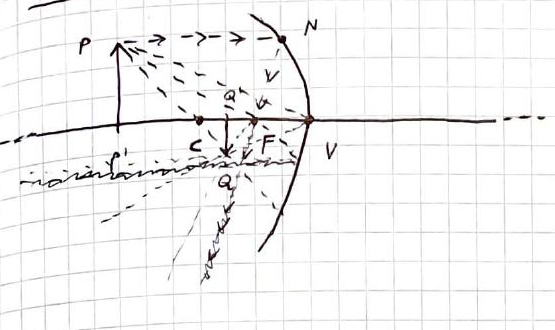
\includegraphics[width=.65\linewidth]{ottica_tex_assets/b36_p38_1.png}\end{center}
Ci sono quattro raggi notevoli:
\begin{enumerate}
\item $P\to N\to F$;
\item $P\to F\to\infty$;
\item $P\to C$;
\item $P\to V$.
\end{enumerate}
Dove si intersecano i quattro raggi notevoli si trova $Q$ ($Q'$ è la proiezione sulla superficie).
\subsubsection*{Ingrandimento trasversale}
\[
I_y=\frac{y'}y=\frac{QQ'}{PP'}.
\]
\[
\begin{gathered}
I_y>1\quad\text{(immagine ingrandita)},\\
I_y<1\quad\text{(immagine rimpicciolita)},\\
I_y=1\quad\text{(immagine coincidente)}.
\end{gathered}
\]
\begin{align*}
I_y&=\frac{QQ'}{PP'}=\frac{CQ}{CP}
=\frac{|R|-|q|}{p-|R|}=\frac{-R+q}{p+R}\\
&=-\frac qp\left(\frac{R/q-1}{1+R/p}\right),\\
\frac1p-\frac1q&=-\frac2R
\quad\Longrightarrow\quad\frac Rp=\frac Rq-2
\quad\Longrightarrow\quad1+\frac Rp=\frac Rq-1,\\
I_y&=-\frac qp\cdot1=-\frac qp.
\end{align*}
\[
I=-\frac qp.
\]
In questo caso $p>0$, $q<0$, quindi $I>0$.
Se $I>0$ l'immagine è capovolta. Se $I<0$ l'immagine è dritta.
% Pagina originale 39
\pagina{39}
\subsubsection*{Specchio piano}
\begin{center}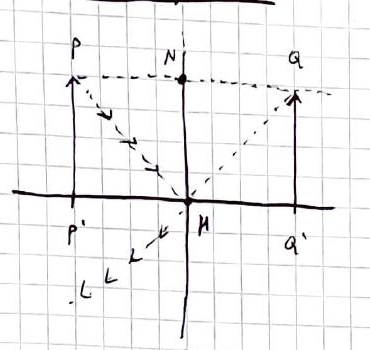
\includegraphics[width=.48\linewidth]{ottica_tex_assets/b36_p39_1.png}\end{center}
Nello specchio piano $R\to\infty$ ($C\to\infty$):
\[
\frac1p-\frac1q=-\frac2R\longrightarrow0
\quad\Longrightarrow\quad p=q,
\qquad I=\frac{y'}y=-\frac qp=-1.
\]
L'immagine non viene ingrandita/rimpicciolita e $I<0$, quindi rimane dritta.
\subsubsection*{Diottro}
Costituito da due mezzi trasparenti con indici di rifrazione diversi, $n_1<n_2$.
\begin{center}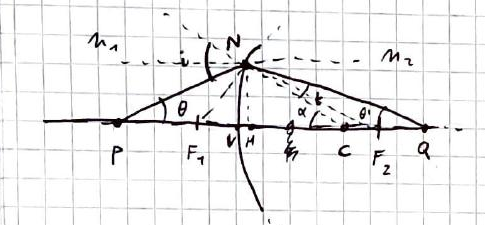
\includegraphics[width=.6\linewidth]{ottica_tex_assets/b36_p39_2.png}\end{center}
\[
i=\theta+\alpha,\qquad\alpha=\theta'+t,
\qquad n_1i=n_2t,\qquad n_1\sin i=n_2\sin t.
\]
\[
n_1(\alpha+\theta)=n_2(\alpha-\theta')
\quad\Longrightarrow\quad
\frac{n_1}{p}+\frac{n_2}{q}=\frac{n_2-n_1}{R}.
\]
Convesso:
\begin{center}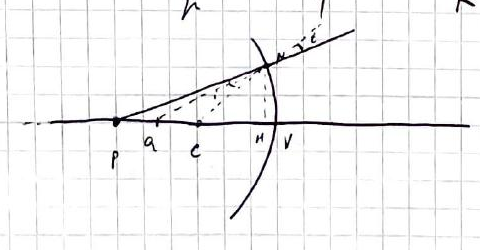
\includegraphics[width=.6\linewidth]{ottica_tex_assets/b36_p39_3.png}\end{center}
\[
\frac{n_1}{p}-\frac{n_2}{q}=-\frac{n_2-n_1}{R}.
\]
\subsubsection*{Convenzione dei segni}
\begin{center}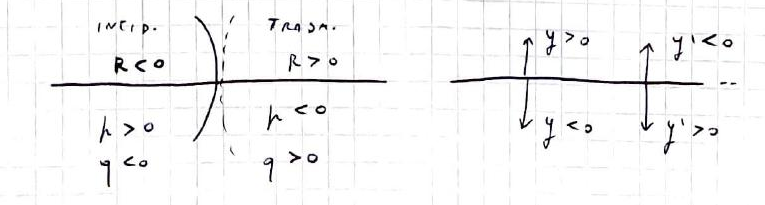
\includegraphics[width=.95\linewidth]{ottica_tex_assets/b36_p39_4.png}\end{center}
Lato incidente: $R<0$, $p>0$, $q<0$; lato trasmesso: $R>0$, $p<0$, $q>0$.
$y>0$ sopra l'asse, $y<0$ sotto; $y'<0$ sopra l'asse, $y'>0$ sotto.
% Pagina originale 40
\pagina{40}
\[
\frac{n_1}{p}+\frac{n_2}{q}=\frac{n_2-n_1}{R}.
\]
Equazione generale: convenzione dei segni.
\subsubsection*{Fuoco}
\[
P\to\infty\quad\Longrightarrow\quad p\to\infty,
\qquad
\frac{n_2}{q}=\frac{n_2-n_1}{R}
\quad\Longrightarrow\quad
q=f_2=\frac{n_2}{n_2-n_1}R.
\]
$f_2$: fuoco posteriore.
\[
Q\to\infty\quad\Longrightarrow\quad q\to\infty,
\qquad
\frac{n_1}{p}=\frac{n_2-n_1}{R}
\quad\Longrightarrow\quad
p=f_1=\frac{n_1}{n_2-n_1}R.
\]
$f_1$: fuoco anteriore.
\begin{center}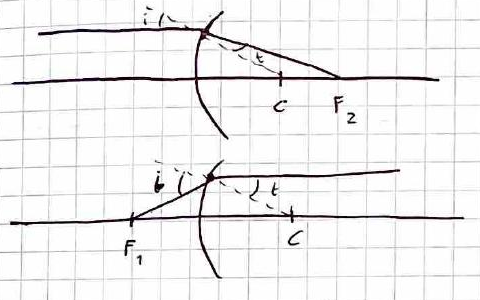
\includegraphics[width=.62\linewidth]{ottica_tex_assets/b36_p40_1.png}\end{center}
Primo caso: $p\to\infty$; secondo caso: $q\to\infty$.
\subsubsection*{Costruzione dell'immagine}
\begin{center}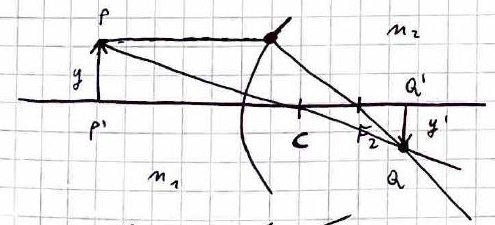
\includegraphics[width=.65\linewidth]{ottica_tex_assets/b36_p40_2.png}\end{center}
\[
I=\frac{y'}y\geq0\quad\Longrightarrow\quad\text{capovolta}
\qquad(y>0,\ y'\geq0).
\]
\begin{center}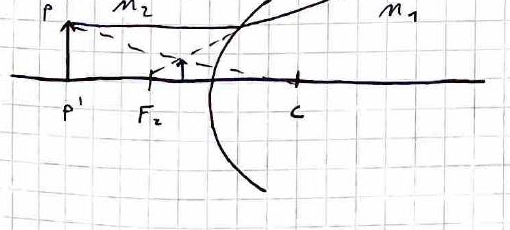
\includegraphics[width=.65\linewidth]{ottica_tex_assets/b36_p40_3.png}\end{center}
\[
I<0\qquad(y>0,\ y'<0),\qquad
I=\frac{n_1q}{n_2p}.
\]
% Pagina originale 41
\pagina{41}
\subsubsection*{Diottro piano}
\begin{center}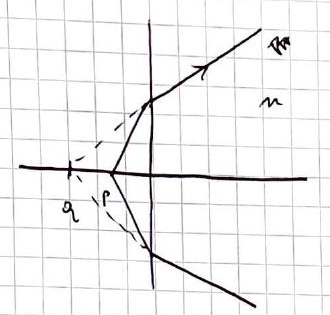
\includegraphics[width=.45\linewidth]{ottica_tex_assets/b36_p41_1.png}\end{center}
\[
\frac{n_1}{p}+\frac{n_2}{q}=\frac{n_2-n_1}{R},
\qquad R\to\infty\quad\Longrightarrow\quad
\frac{n_1}{p}=-\frac{n_2}{q}
\quad\Longrightarrow\quad q=-\frac{n_2}{n_1}p.
\]
\[
I=\frac{n_1q}{n_2p}
=\frac{n_1\left(-\frac{n_2}{n_1}p\right)}{n_2p}=-1<0.
\]
\subsubsection*{Lenti}
È l'insieme di due diottri.
\begin{center}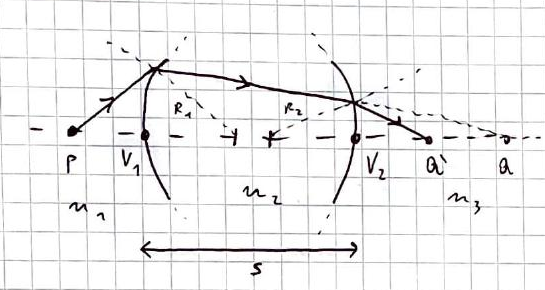
\includegraphics[width=.75\linewidth]{ottica_tex_assets/b36_p41_2.png}\end{center}
\[
\frac{n_1}{p_1}+\frac{n_2}{q_1}=\frac{n_2-n_1}{R_1},\qquad
\frac{n_2}{p_2}+\frac{n_3}{q_2}=\frac{n_3-n_2}{R_2},\qquad p_2=s-q_1.
\]
\[
n_1=n_3\quad\Longrightarrow\quad
\frac{n_1}{p_1}+\frac{n_2s}{q_1(s-q_1)}+\frac{n_1}{q_2}
=(n_2-n_1)\left(\frac1{R_1}-\frac1{R_2}\right).
\]
\subsubsection*{Lenti sottili}
\begin{center}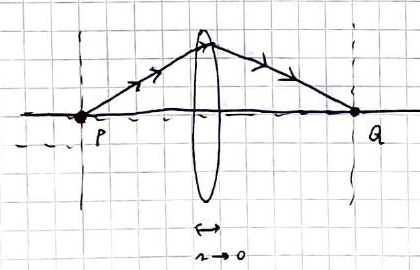
\includegraphics[width=.58\linewidth]{ottica_tex_assets/b36_p41_3.png}\end{center}
\[
s\to0,\qquad
\frac{n_1}{p_1}+\frac{n_1}{q_2}
=(n_2-n_1)\left(\frac1{R_1}-\frac1{R_2}\right),
\qquad p_1=p,\quad q_1=q.
\]
% Nella riga manoscritta prima dell'ultima formula l'indice di q appare 1; la formula precedente usa q_2. Si conserva q_1 nell'annotazione originale:

\[
\frac1p+\frac1q=\frac{n_2-n_1}{n_1}
\left(\frac1{R_1}-\frac1{R_2}\right)=\frac1f.
\]
% Pagina originale 42
\pagina{42}
\subsubsection*{Classificazione delle lenti}
\begin{center}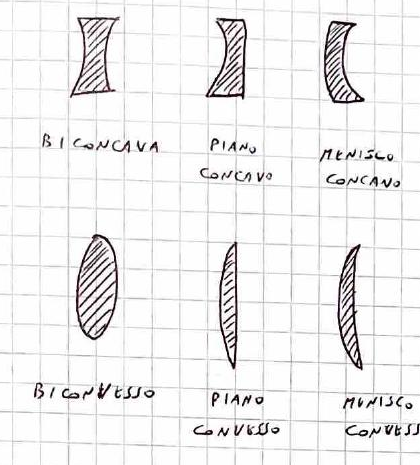
\includegraphics[width=.7\linewidth]{ottica_tex_assets/b36_p42_1.png}\end{center}
Divergenti: biconcava, piano-concava, menisco concavo; $1/f<0$.
Convergenti: biconvessa, piano-convessa, menisco convesso; $1/f>0$.
\subsubsection*{Lente convergente}
\begin{center}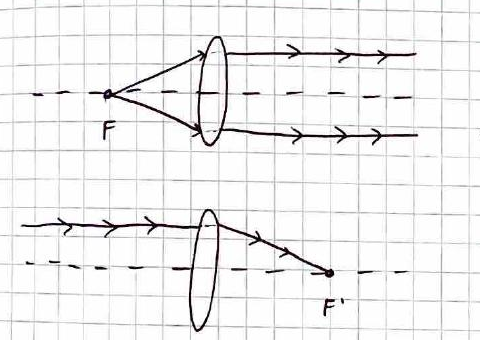
\includegraphics[width=.7\linewidth]{ottica_tex_assets/b36_p42_2.png}\end{center}
\[
q\to\infty\quad\Longrightarrow\quad p=f,
\qquad q\to\infty\quad\Longrightarrow\quad p=f,
\qquad p\to\infty\quad\Longrightarrow\quad q=f,
\qquad\frac1p+\frac1q=\frac1f.
\]
% La prima relazione q -> infinito è ripetuta due volte nella pagina originale.
\subsubsection*{Lente divergente}
\begin{center}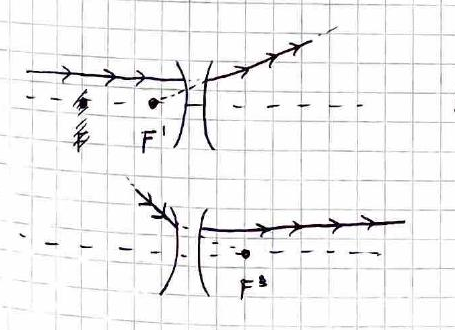
\includegraphics[width=.7\linewidth]{ottica_tex_assets/b36_p42_3.png}\end{center}
\[
p\to\infty\quad\Longrightarrow\quad q=f,
\qquad q\to\infty\quad\Longrightarrow\quad p=f.
\]
La distanza focale è sempre uguale:
\[
\frac1f=\frac1{f'}.
\]
% Pagina originale 43
\pagina{43}
\[
\frac1f=P\qquad\text{potenza (potere diottrico)}.
\]
È l'inverso della distanza focale. Unità di misura: $D$, diottrie,
\[
D=\frac1{\mathrm m}=\mathrm m^{-1}.
\]
$P>0$ per lenti convergenti; $P<0$ per lenti divergenti.
\subsubsection*{Costruzione dell'immagine}
\begin{center}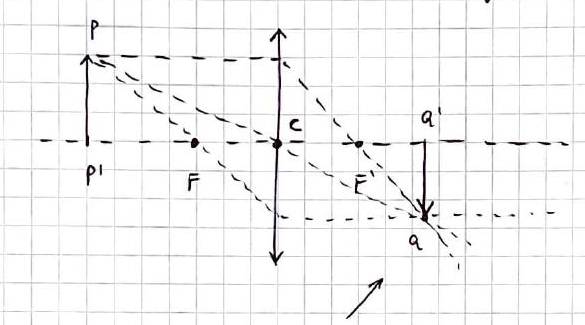
\includegraphics[width=.8\linewidth]{ottica_tex_assets/b36_p43_1.png}\end{center}
I raggi sono:
\begin{enumerate}
\item $P\to F'$;
\item $P\to F$: parallelo;
\item $P\to C$.
\end{enumerate}
Immagine reale e capovolta.
\begin{center}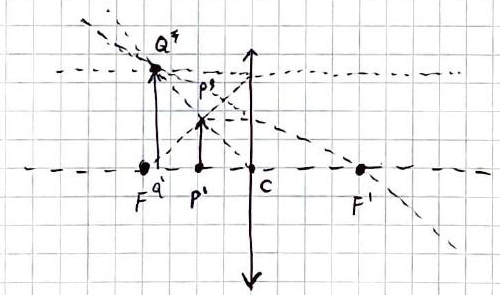
\includegraphics[width=.7\linewidth]{ottica_tex_assets/b36_p43_2.png}\end{center}
$P\in(F,C)$: immagine virtuale e dritta.
\begin{center}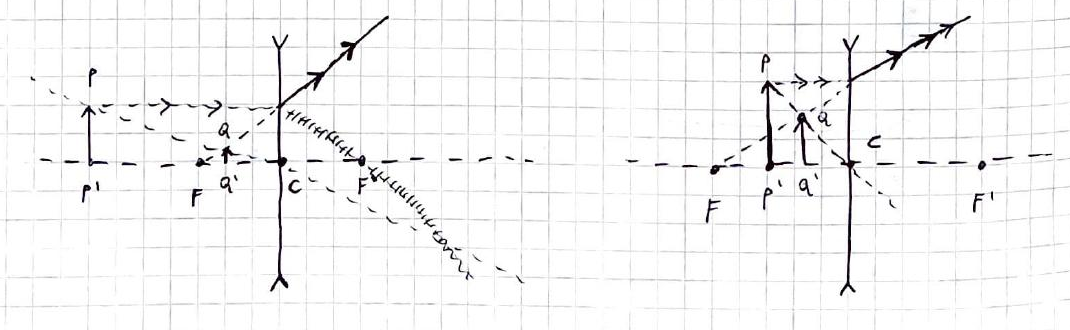
\includegraphics[width=\linewidth]{ottica_tex_assets/b36_p43_3.png}\end{center}
Nei due casi rappresentati: immagine virtuale e dritta.
% Pagina originale 44
\pagina{44}
\subsubsection*{Ingrandimento}
\[
I=\frac qp=\frac{q-f}{q}=\frac f{p-f}.
\]
% La frazione intermedia (q-f)/q è quella manoscritta, benché non coincida in generale con q/p.
\subsubsection*{Sistema di lenti}
\[
\text{Oggetto}_1\xrightarrow{\text{lente 1}}\text{Immagine}_1
=\text{Oggetto}_2\xrightarrow{\text{lente 2}}\text{Immagine}_2.
\]
Si può dimostrare che
\[
\frac1{f_{\mathrm{eq}}}=\frac1{f_1}+\frac1{f_2},\qquad
P_{\mathrm{eq}}=\sum_i P_i.
\]
Le lenti si dicono \emph{addossate} se la loro distanza è nulla o trascurabile.
\begin{center}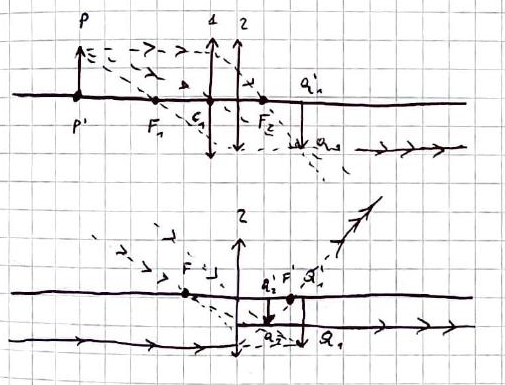
\includegraphics[width=.7\linewidth]{ottica_tex_assets/b36_p44_1.png}\end{center}
$Q_1$ è un'immagine virtuale che diventa oggetto virtuale per la lente 2. $Q_2$ è l'immagine finale.
\begin{align*}
\frac1{p_1}+\frac1{q_1}&=\frac1{f_1},\\
\frac1{p_2}+\frac1{q_2}&=-\frac1{q_1}+\frac1{q_2}=\frac1{f_2}.
\end{align*}
\[
\begin{cases}\frac1p+\frac1{q_1}=\frac1{f_1},\\
\frac1q-\frac1{q_1}=\frac1{f_2},\end{cases}
\quad\Longrightarrow\quad
\frac1p+\frac1q=\frac1{f_1}+\frac1{f_2}
\quad\Longrightarrow\quad
\frac1f=\frac1{f_1}+\frac1{f_2}.
\]
% Pagina originale 45
\pagina{45}
\subsubsection*{Occhio}
\begin{itemize}
\item Coroide: assorbe la luce dispersa.
\item Cornea: devia gran parte della luce.
\item Umor acqueo: liquido tra cornea e cristallino (indice $n$: valore tagliato al margine destro, pagina 45).
\item Pupilla: determina la quantità di luce che entra nell'occhio.
\item Cristallino: lente biconvessa con $n\simeq1{,}47$.
\item Umor vitreo: sostanza gelatinosa tra cristallino e retina ($n\simeq1{,}33$).
\end{itemize}
Potere diottrico:
\[
P_0=60\,D\quad\Longrightarrow\quad f=\frac1D=17\,\mathrm{mm}.
\]
\subsubsection*{Immagini reali e virtuali}
\paragraph{Specchi}
\[
\frac1p-\frac1q=-\frac2R.
\]
\begin{itemize}
\item Piani: sempre virtuale, dritta, $I=-1$.
\item Concavi: reale se $p>f$, immagine capovolta; virtuale se $p<f$, immagine dritta.
\item Convessi: sempre virtuale, dritta, $|I|<1$.
\end{itemize}
Negli specchi è reale se lo specchio è concavo e $p>f$.
\paragraph{Lenti}
\[
\frac1p+\frac1q=\frac1f.
\]
\begin{itemize}
\item Convergenti: reale se $p>f\Rightarrow q>0$; virtuale se $p<f\Rightarrow q<0$.
\item Divergenti: sempre virtuale ($q<0$), dritta, $|I|<1$.
\end{itemize}
\paragraph{Diottri}
\[
\frac{n_1}{p}+\frac{n_2}{q}=\frac{n_2-n_1}{R},\qquad
q<0\ \longrightarrow\ \text{virtuale},\qquad
q>0\ \longrightarrow\ \text{reale}.
\]
% Pagina originale 46
\pagina{46}
\subsubsection*{Interferenza}
\begin{center}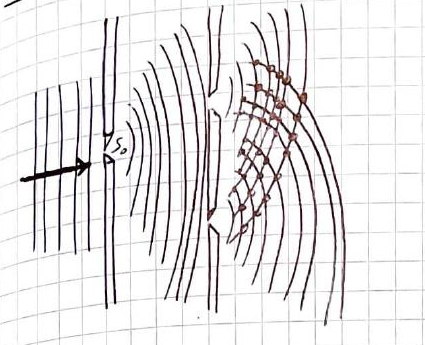
\includegraphics[width=.55\linewidth]{ottica_tex_assets/b36_p46_1.png}\end{center}
\begin{align*}
\vv E_1(r,t)&=\frac{\vv E_0}{r}\sin(kr-\omega t+\phi_1),\\
\vv E_2(r,t)&=\frac{\vv E_0}{r}\sin(kr-\omega t+\phi_2),\\
\delta&=k(r_2-r_1)+(\phi_2-\phi_1)\qquad\text{differenza di fase}.
\end{align*}
Se $\Delta\phi=0$, allora $\delta=k(r_2-r_1)$.
\begin{center}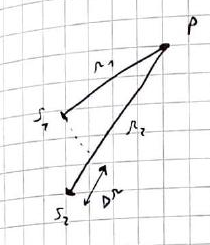
\includegraphics[width=.3\linewidth]{ottica_tex_assets/b36_p46_2.png}\end{center}
Se $\partial\delta/\partial t=0$ (costante nel tempo) le sorgenti si dicono coerenti.
\[
\frac{\partial\delta}{\partial t}\ne0\quad\Longrightarrow\quad\text{sorgenti incoerenti}.
\]
\subsubsection*{Esperimento di Young}
\begin{center}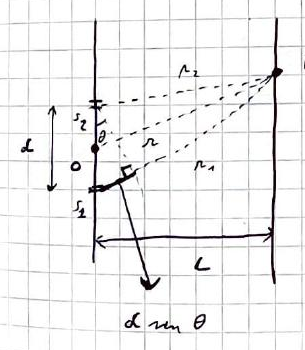
\includegraphics[width=.43\linewidth]{ottica_tex_assets/b36_p46_3.png}\end{center}
Prendiamo due onde sferiche con stessa lunghezza d'onda (quindi stesso $k$):
\[
\vv E_1(r,t)=\frac{\vv E_0}{r}\sin(kr-\omega t),\qquad
\vv E_2(r,t)=\frac{\vv E_0}{r}\sin(kr-\omega t).
\]
\begin{align*}
\vv E_P&=\vv E_1(r,t')+\vv E_2(r,t')\\
&=\frac{\vv E_0}{r_1}\sin(kr_1-\omega t')+
\frac{\vv E_0}{r_2}\sin(kr_2-\omega t').
\end{align*}
Poniamo $r\simeq r_1\simeq r_2$:
\[
\vv E_P=\frac{\vv E_0}{r}\left[
\sin\left(\frac{kr_1-\omega t'+kr_2-\omega t'}2\right)
\cos\left(\frac{kr_1-\omega t'-kr_2+\omega t'}2\right)
\right].
\]
% La formula manoscritta non mostra il fattore 2 della somma di seni; conservata.
% Pagina originale 47
\pagina{47}
Sfruttando la formula di sovrapposizione:
\begin{align*}
A\left[\sin(k_1x-\omega_1t)+\sin(k_2x-\omega_2t)\right]
&=2A\cos\left(\frac{\Delta k}{2}x-\frac{\Delta\omega}{2}t\right)
\sin(k_mx-\omega_mt),
\end{align*}
$k_m$, $\omega_m$: medie. Quindi
\[
\vv E_P=2\frac{\vv E_0}{r}
\sin\left(\frac{k(r_1+r_2)}2-\omega t'\right)
\cos\left(\frac{k(r_1-r_2)}2\right).
\]
\[
\frac{r_1+r_2}{2}\simeq r,\qquad\delta=k(r_1-r_2),
\]
\[
\vv E_P=2\frac{\vv E_0}{r}\sin(kr-\omega t')\cos\frac\delta2,
\quad\text{cioè}\quad
\vv E_P=2\frac{\vv E_0}{r}\cos\frac\delta2\cdot\sin(kr-\omega t'),
\qquad |\vv E_P|=2\frac{E_0}{r}\cos\frac\delta2.
\]
\begin{align*}
I&=c\varepsilon_0\langle E_P^2\rangle
=c\varepsilon_0\left[2\frac{E_0}{r}\cos\frac\delta2\right]^2
\langle\sin^2(kr-\omega t')\rangle\\
&=\frac12\,4\frac{E_0^2}{r^2}\cos^2\frac\delta2\,c\varepsilon_0
=4\frac{I_0}{r^2}\cos^2\frac\delta2
\qquad(I\propto\delta).
\end{align*}
\[
\delta=k(r_1-r_2)=\frac{2\pi}{\lambda}(r_1-r_2),\qquad
r_1-r_2\simeq d\sin\theta.
\]
\begin{align*}
I&=4\frac{I_0}{r^2}\cos^2\frac\delta2\simeq4I_0\cos^2\frac\delta2\\
&=4I_0\cos^2\left(\frac{kd\sin\theta}2\right)
=4I_0\cos^2\left(\frac{\pi d\sin\theta}{\lambda}\right).
\end{align*}
\[
I_{\max}=4I_0\quad\Longrightarrow\quad
\frac{\pi d\sin\theta}{\lambda}=m\pi,
\qquad
I_{\min}=0\quad\Longrightarrow\quad
\frac{\pi d\sin\theta}{\lambda}=\left(m+\frac12\right)\pi.
\]
% Si conserva il passaggio approssimato che assorbe 1/r^2 in I_0 e l'annotazione I proporzionale a delta dell'originale.
% Pagina originale 48
\pagina{48}
Cioè
\[
d\sin\theta=m\lambda\quad\text{massimi},\qquad
d\sin\theta=\left(m+\frac12\right)\lambda\quad\text{minimi}.
\]
Se $L\gg d$:
\[
\sin\theta\simeq\tan\theta\simeq\theta=\frac xL,
\qquad I(x)=4I_0\cos^2\left(\frac{\pi d}{\lambda L}x\right).
\]
Quindi
\begin{align*}
x_M&=\frac Ld m\lambda
\quad\Longrightarrow\quad
\theta_M=\frac{x_M}{L}=\frac Ld m\lambda\cdot\frac1L,\\
x_m&=\frac Ld\left(m+\frac12\right)\lambda
\quad\Longrightarrow\quad
\theta_m=\frac{x_m}{L}=\frac{L\lambda}{d}\left(m+\frac12\right)\frac1L.
\end{align*}
\[
\theta_M=\frac\lambda d m,\qquad
\theta_m=\frac\lambda d\left(m+\frac12\right).
\]
\begin{center}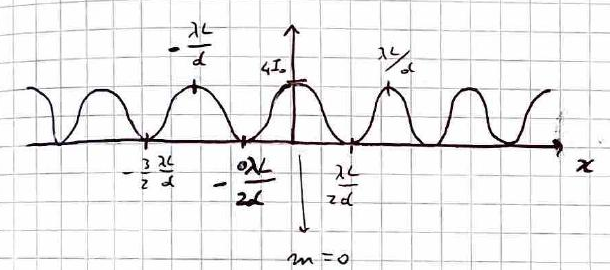
\includegraphics[width=.82\linewidth]{ottica_tex_assets/b36_p48_1.png}\end{center}
I passi
\[
p_M=x_{M+1}-x_M=\frac{\lambda L}{d}
\]
sono le distanze tra due frange chiare (massimi).
Se le onde si propagano in un mezzo con indice di rifrazione $n$:
\[
\delta=kn(r_1-r_2)=\frac{2\pi}{\lambda}nd\sin\theta,
\]
\[
I(\theta)=4I_0\cos^2\left(n\frac{\pi d\sin\theta}{\lambda}\right),\qquad
I(x)=4I_0\cos^2\left(n\frac{\pi dx}{\lambda L}\right).
\]
% Pagina originale 49
\pagina{49}
\subsubsection*{Sorgenti incoerenti}
\[
\delta=k(r_2-r_2)+(\phi_2-\phi_1)
=k(r_2-r_1)+\Delta\phi(t).
\]
% Il primo termine manoscritto sembra r_2-r_2, mentre nella stessa riga è poi r_2-r_1; refuso conservato.
\[
\vv E_P=\left[2\frac{\vv E_0}{r}\cos\left(\frac{\delta+\Delta\phi(t)}2\right)\right]
\sin(kr-\omega t').
\]
\begin{align*}
I&=c\varepsilon_0\langle E_P^2\rangle
=c\varepsilon_0\left[2\frac{E_0}{r}\right]^2
\left\langle\cos^2\left(\frac{\delta+\Delta\phi(t)}2\right)\right\rangle
\langle\sin^2(kr-\omega t')\rangle\\
&=c\varepsilon_0\,4\frac{E_0^2}{r^2}\cdot\frac12\cdot\frac12
=2\frac{I_0}{r^2}.
\end{align*}
\[
I=2I_0\frac1{r^2}\qquad\text{costante e non dipendente da }x.
\]
\subsubsection*{Effetto cromatico}
\[
I(\theta)=4I_0\cos^2\left(\frac{\pi d\sin\theta}{\lambda}\right)
\propto\cos^2\frac{\cdots}{\lambda}.
\]
Dipende da $\lambda$.
\[
x(\lambda)=m\frac{\lambda L}{d}
\]
Cambia per ogni colore: $x_{m=1,\mathrm{rosso}}\ne x_{m=1,\mathrm{blu}}$, ecc.
\begin{center}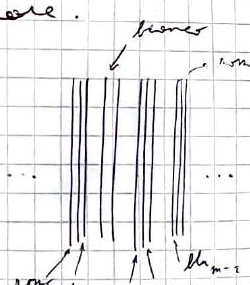
\includegraphics[width=.38\linewidth]{ottica_tex_assets/b36_p49_1.png}\end{center}
\subsubsection*{Lamine sottili}
\begin{center}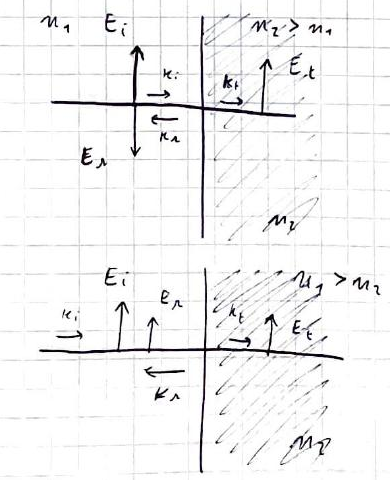
\includegraphics[width=.52\linewidth]{ottica_tex_assets/b36_p49_2.png}\end{center}
Se $n_2>n_1$: $r_0<0$ (sfasato di $\pi$), $t_0>0$ (in fase).
Se $n_1>n_2$: $r_0>0$, $t_0>0$ (in fase).
% Pagina originale 50
\pagina{50}
\begin{center}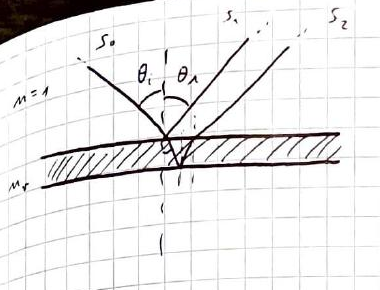
\includegraphics[width=.55\linewidth]{ottica_tex_assets/b36_p50_1.png}\end{center}
\[
\delta=k(r_1-r_2)+\Delta\phi(t),\qquad
\phi_1=\phi_0+\pi\quad(n>1),\qquad\phi_2=\phi_0.
\]
\[
\phi_2-\phi_1=\phi_0-(\phi_0+\pi)=-\pi=\Delta\phi.
\]
\begin{align*}
\delta&=k(r_2-r_1)+\Delta\phi=k(2nd\cos\theta_r)-\pi\\
&=2kd\sqrt{n^2-\sin^2\theta_i}-\pi.
\end{align*}
Quando c'è incidenza normale, $\theta_i=\theta_r=0$:
\[
\delta=2kdn-\pi=\frac{4\pi dn}{\lambda}-\pi.
\]
\begin{align*}
I&=4I_0\cos^2\frac\delta2
=4I_0\cos^2\left(\frac{4\pi dn}{\lambda}-\pi\right)\\
&=4I_0\left[-\cos\left(\frac{4\pi dn}{\lambda}\right)\right]^2
=4I_0\cos^2\left(\frac{2\pi dn}{\lambda}\right).
\end{align*}
% I passaggi intermedi del manoscritto omettono la divisione per 2 dell'argomento; conservati senza correzioni silenziose.
\[
\frac\delta2=m\pi\qquad\text{interferenza costruttiva},\qquad
\frac\delta2=\left(m+\frac12\right)\pi\qquad\text{interferenza distruttiva}.
\]
\[
d=\left(m+\frac12\right)\frac\lambda{2n}\quad\text{I.C.},\qquad
d=m'\frac\lambda{2n}\quad\text{I.D.}
\]
\subsubsection*{Cuneo sottile}
\begin{center}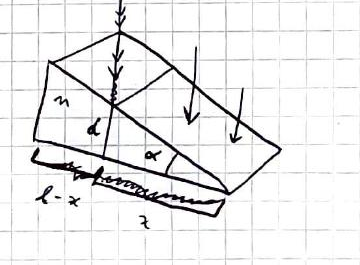
\includegraphics[width=.55\linewidth]{ottica_tex_assets/b36_p50_2.png}\end{center}
Se $\alpha\simeq0$, allora
\[
\tan\alpha\simeq\alpha=\frac dx.
\]
Trattiamo il cuneo come una lamina sottile.
% Pagina originale 51
\pagina{51}
\[
d=\left(m+\frac12\right)\frac\lambda{2n}
\quad\Longrightarrow\quad
\alpha=\left(m+\frac12\right)\frac\lambda{2nx}
\quad\Longrightarrow\quad
x=\left(m+\frac12\right)\frac\lambda{2n\alpha}\quad\text{I.C.}
\]
\[
x=m'\frac\lambda{2n\alpha}\qquad\text{I.D.}
\]
\subsubsection*{Anelli di Newton}
\begin{center}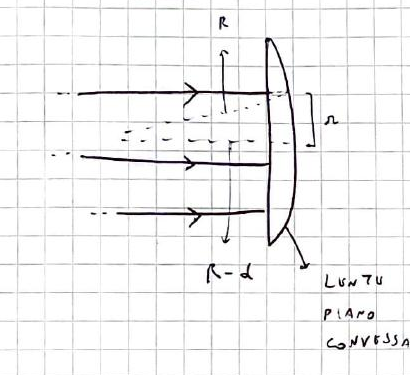
\includegraphics[width=.5\linewidth]{ottica_tex_assets/b36_p51_1.png}\end{center}
Lente piano-convessa:
\begin{align*}
r^2&=R^2-(R-d)^2=-d^2+2Rd,\\
\frac{r^2}{4R^2}&=\frac d{2R}-\left(\frac d{2R}\right)^2,\\
d\ll R&\quad\Longrightarrow\quad\frac{r^2}{4R^2}=\frac d{2R}
\quad\Longrightarrow\quad r^2=2Rd.
\end{align*}
Il sistema è simile al cuneo.
\[
d=\left(m+\frac12\right)\frac\lambda{2n}
\quad\Longrightarrow\quad
r^2=\left(m+\frac12\right)\frac{2R\lambda}{2n}.
\]
\[
r=\sqrt{\left(m+\frac12\right)R\lambda}\quad\text{I.C.},\qquad
r=\sqrt{m'R\lambda}\quad\text{I.D.}
\]
% Le ultime espressioni originali non riportano il fattore 1/n.
\subsubsection*{Interferenza di $N$ sorgenti}
\begin{center}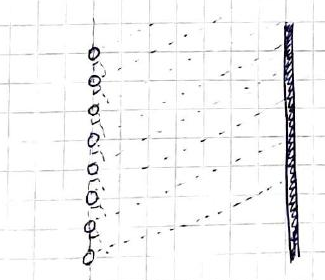
\includegraphics[width=.42\linewidth]{ottica_tex_assets/b36_p51_2.png}\end{center}
\[
\delta=k(r_i-r_{i+1})=\frac{2\pi}{\lambda}(r_i-r_{i+1}),
\qquad
\vv E_0=\vv E_0\sin(kx-\omega t),\qquad
\vv E_i=\vv E_0\sin(kx-\omega t+i\delta).
\]
% Pagina originale 52
\pagina{52}
\begin{align*}
\vv E_P(r,t)&=\vv E_1(r,t)+\vv E_2(r,t)+\cdots+\vv E_N(r,t),\\
\vv E_P(r,t)&=\sum_{i=1}^{N}\vv E_i(r,t)
=\vv E_0\sum_{i=1}^{N}\sin(kr-\omega t+i\delta).
\end{align*}
Trattiamo i moduli:
\[
E_0=2\rho\sin\frac\delta2,\qquad E_P=2\rho\sin\frac{N\delta}{2}.
\]
\[
E_P=E_0\frac{\sin(N\delta/2)}{\sin(\delta/2)}
\quad\Longrightarrow\quad
I_P=I_0\frac{\sin^2(N\delta/2)}{\sin^2(\delta/2)}.
\]
Calcoliamo $\delta$:
\[
\delta=k(r_i-r_{i+1})=\frac{2\pi}{\lambda}d\sin\theta.
\]
\[
I_P(\theta)=I_0\frac{\sin^2(N\delta/2)}{\sin^2(\delta/2)}
=I_0\left[\frac{\sin(\pi Nd\sin\theta/\lambda)}
{\sin(\pi d\sin\theta/\lambda)}\right]^2.
\]
Se $N=2$:
\[
I_P(\theta)=I_0\frac{\left(2\sin\frac\delta2\cos\frac\delta2\right)^2}
{\left(\sin\frac\delta2\right)^2}=4I_0\cos^2\frac\delta2.
\]
\begin{center}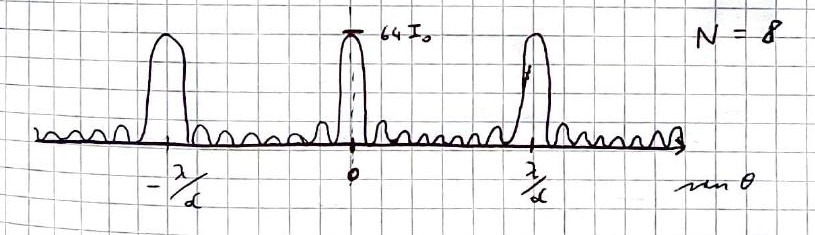
\includegraphics[width=\linewidth]{ottica_tex_assets/b36_p52_1.png}\end{center}
$N=8$, massimo centrale $64I_0$; ascissa $\sin\theta$, massimi a $-\lambda/d$, $0$, $\lambda/d$.
\[
\lim_{\delta\to0}I_0\frac{\sin^2(N\delta/2)}{\sin^2(\delta/2)}
=\lim_{\delta\to0}I_0\frac{N^2\delta^2/4}{\delta^2/4}=I_0N^2.
\]
$I_{\max}$: massimi principali.
I massimi principali si hanno quando il denominatore tende a zero:
\[
\Delta(\sin\theta)_{\max}=\frac\lambda d,
\]
\[
I_M=\lim_{\frac\pi\lambda d\sin\theta\to m\pi}
I_0\frac{\sin^2(N\pi d\sin\theta/\lambda)}
{\sin^2(\pi d\sin\theta/\lambda)}=N^2I_0.
\]
% Pagina originale 53
\pagina{53}
Il minimo si ha quando il numeratore tende a zero (e il denominatore non è diverso da zero, come scritto negli appunti).
% L'inciso originale «den. non è diverso da 0» è conservato, pur essendo incoerente con la condizione sui minimi.
\[
\sin^2\left(\frac{N\pi}{\lambda}d\sin\theta\right)\to0
\quad\Longrightarrow\quad\frac{N\pi}{\lambda}d\sin\theta\to0,
\]
\[
\sin\theta\,\frac{N\pi}{\lambda}d=m'\pi
\quad\Longrightarrow\quad\sin\theta=\frac{m'\lambda}{Nd}.
\]
\[
(\sin\theta)_{\min}=(\sin\theta)_{\max}
\quad\Longleftrightarrow\quad m'\frac\lambda{Nd}=m\frac\lambda d
\quad\Longrightarrow\quad m'=Nm.
\]
$m'$ non è un minimo ma un massimo.
I massimi secondari si hanno quando il seno è 1:
\[
\sin^2\left(\frac{N\pi}{\lambda}d\sin\theta\right)=1
\quad\Longrightarrow\quad
\frac{N\pi}{\lambda}d\sin\theta=\left(m''+\frac12\right)\pi\lambda,
\]
% L'ultima lambda della riga manoscritta è conservata; il passaggio seguente non la include.
\[
\sin\theta=\left(m''+\frac12\right)\frac\lambda{Nd},
\qquad m''=0,\pm1,\pm2,\ldots
\]
\[
I''=\frac{I_0}{\sin^2\left((m''+\frac12)\frac\pi N\right)}
=\frac{I_M}{N^2\sin^2\left((m''+\frac12)\frac\pi N\right)}.
\]
\[
(\sin\theta)_{m'=1}=\frac\lambda{Nd},\qquad
(\sin\theta)_{m'=-1}=-\frac\lambda{Nd},\qquad
\Delta(\sin\theta)=\frac{2\lambda}{Nd}.
\]
Larghezza angolare dei massimi principali:
\begin{center}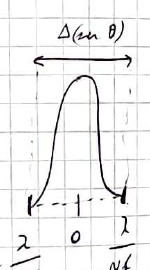
\includegraphics[width=.3\linewidth]{ottica_tex_assets/b36_p53_1.png}\end{center}
\subsubsection*{Caratteristiche}
\begin{itemize}
\item $m=0$: massimo principale.
\item Tra due massimi principali ci sono $N-2$ massimi secondari.
\item Tra due massimi principali ci sono $N-1$ minimi.
\item $I_{\max,\mathrm{pr}}=N^2I_0$.
\item Ampiezza angolare $\propto1/N$.
\item $I_{\max,\mathrm{sec}}\propto\frac1{N^2}I_{\max,\mathrm{pr}}$
($I_{\max,\mathrm{sec}}\simeq I_0$).
\end{itemize}
% Pagina originale 54
\pagina{54}
\begin{center}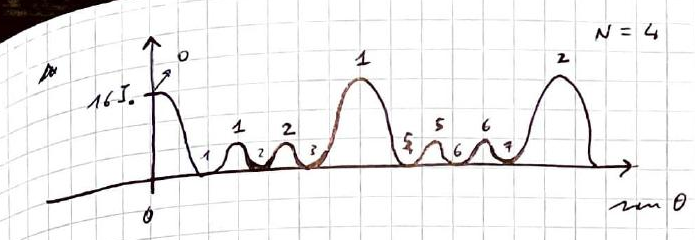
\includegraphics[width=.85\linewidth]{ottica_tex_assets/b36_p54_1.png}\end{center}
$N=4$:
\[
\text{max P}:\ \sin\theta=m\frac\lambda d,\qquad
\text{max S}:\ \sin\theta=\left(m''+\frac12\right)\frac\lambda{Nd},\qquad
\text{min}:\ \sin\theta=m'\frac\lambda{Nd}.
\]
\begin{center}\small
\begin{tabular}{c|*{11}{c}}
$\frac d\lambda\sin\theta$&0&$\frac18$&$\frac28$&$\frac38$&$\frac12$&$\frac58$&$\frac34$&$\frac78$&1&$\frac98$&$\frac54$\\\hline
$m$, max P&0&&&&&&&&1&&\\
$m''$, max S&&0&&1&&2&&3&&4&\\
$m'$, min&0&&1&&2&&3&&4&&5
\end{tabular}
\end{center}
$m'=0$ e $m'=4$ per i minimi non sono valori validi perché $m'=Nm$ ($m'$ multiplo di $N$).
$m''=0$, $m''=3$, $m''=4$ non sono validi perché compresi tra il massimo principale ed il primo minimo (o tra l'ultimo minimo e il massimo principale).
\subsubsection*{Diffrazione}
La diffrazione è una particolare interferenza che avviene quando le dimensioni dell'ostacolo sono prossime alla lunghezza d'onda della radiazione.
Esistono due tipi di diffrazione:
\begin{itemize}
\item Fresnel: campo vicino;
\item Fraunhofer: campo lontano.
\end{itemize}
% Pagina originale 55
\pagina{55}
\subsubsection*{Diffrazione di Fraunhofer: fenditura singola}
\begin{center}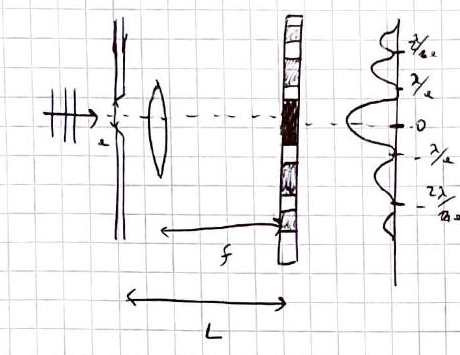
\includegraphics[width=.62\linewidth]{ottica_tex_assets/b36_p55_1.png}\end{center}
Divido la fenditura in $N$ sorgenti:
\[
\Delta y=\frac aN,\qquad
\Delta\phi=\frac{2\pi}{\lambda}\Delta y\sin\theta
\quad[=k(y_i-y_{i+1})].
\]
\[
\alpha=\frac{2\pi}{\lambda}a\sin\theta
\qquad\text{è la differenza di fase totale}.
\]
\[
\begin{cases}E_P=2\rho\sin\frac\alpha2,\\E_{\max}=\rho\alpha,\end{cases}
\quad\Longrightarrow\quad E_P=2\frac{E_{\max}}\alpha\sin\frac\alpha2.
\]
\[
E_P(\theta)=E_{\max}\frac{\sin(\alpha/2)}{\alpha/2}
=E_{\max}\frac{\sin(\frac\pi\lambda a\sin\theta)}
{\frac\pi\lambda a\sin\theta}.
\]
\[
I_P(\theta)=I_{\max}\left(\frac{\sin(\frac\pi\lambda a\sin\theta)}
{\frac\pi\lambda a\sin\theta}\right)^2.
\]
\[
I_P=I_{\max}\quad\text{se}\quad\frac\pi\lambda a\sin\theta\to0.
\]
Questa condizione si realizza solo quando $\theta=0$ e si parla di massimo centrale.
I minimi si hanno quando si annulla il numeratore:
\[
\frac\pi\lambda a\sin\theta=m\pi
\quad\Longrightarrow\quad\sin\theta=m\frac\lambda a,
\qquad m=\pm1,\pm2,\ldots
\]
I massimi secondari si hanno quando il seno è 1:
\[
\frac\pi\lambda a\sin\theta=\left(m'+\frac12\right)\pi
\quad\Longrightarrow\quad
\sin\theta=\left(m'+\frac12\right)\frac\lambda a,\qquad m'=1,2,\ldots
\]
% Pagina originale 56
\pagina{56}
\[
\frac{I_P}{I_{\max}}=\frac1{\pi^2(m'+\frac12)^2}.
\]
Con $m'=1$: $I_{\mathrm{sec},P}=0{,}045I_{\max}$.
La maggior parte della potenza si trova nella frangia centrale ($\simeq80\%$).
\[
\Delta(\sin\theta)=2\frac\lambda a
\quad\Longrightarrow\quad
\Delta\theta=2\frac\lambda{a\cos\theta}
\xrightarrow{\theta\simeq0}\Delta\theta=2\frac\lambda a.
\]
\subsubsection*{Diffrazione da apertura circolare}
Primo minimo di intensità:
\[
\sin\theta=1{,}22\frac\lambda D,
\qquad D:\ \text{diametro}.
\]
La larghezza angolare del massimo è $2\theta=\phi$.
\subsubsection*{Criterio di Rayleigh}
Due figure di diffrazione sono risolte se il massimo centrale di una cade nel primo zero dell'altra.
\subsubsection*{Interferenza e diffrazione: doppia fenditura sottile}
\begin{center}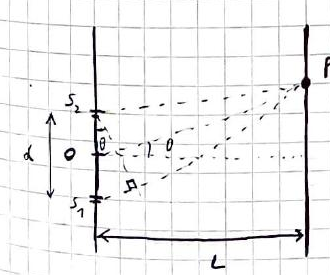
\includegraphics[width=.48\linewidth]{ottica_tex_assets/b36_p56_1.png}\end{center}
\[
E_{P1}(\theta)=E_0\frac{\sin(\frac\pi\lambda a\sin\theta)}
{\frac\pi\lambda a\sin\theta},\qquad
E_{P2}(\theta)=E_0\frac{\sin(\frac\pi\lambda a\sin\theta)}
{\frac\pi\lambda a\sin\theta}.
\]
Uso Carnot:
\begin{align*}
E_P^2&=E_{P1}^2+E_{P2}^2-2E_{P1}E_{P2}\cos(\pi-\delta)\\
&=E_{P1}^2+E_{P2}^2+2E_{P1}E_{P2}\cos\delta.
\end{align*}
% Pagina originale 57
\pagina{57}
Con $I=\frac12c\varepsilon_0 E^2$:
\[
I_P=2I_0\left[\frac{\sin(\frac\pi\lambda d\sin\theta)}
{\frac\pi\lambda a\sin\theta}\right]^2(1+\cos\delta)
=4I_0\left[\frac{\sin(\frac\pi\lambda a\sin\theta)}
{\frac\pi\lambda a\sin\theta}\right]^2\cos^2\frac\delta2.
\]
% Nel primo numeratore la lettera manoscritta è d; nella forma finale è a. Si conservano entrambe.
\[
\delta=\frac{2\pi d\sin\theta}{\lambda},\qquad
I_{\max}=N^2I_0.
\]
\[
I_P=I_{\max}
\underbrace{\left(\frac{\sin(\frac\pi\lambda a\sin\theta)}
{\frac\pi\lambda a\sin\theta}\right)^2}_{\text{fattore di diffrazione}}
\underbrace{\cos^2\left(\frac\pi\lambda d\sin\theta\right)}_{\text{fattore di interferenza}}.
\]
\paragraph{Esempio}
\begin{center}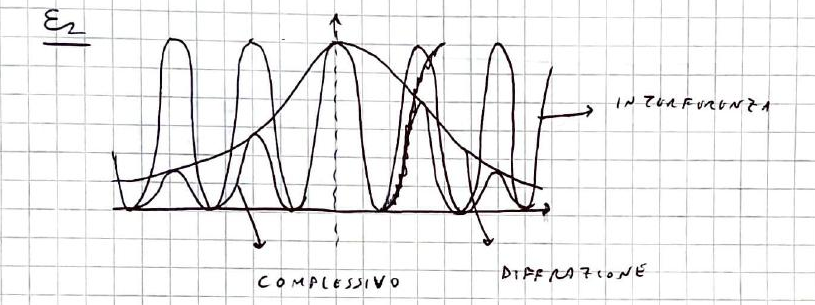
\includegraphics[width=\linewidth]{ottica_tex_assets/b36_p57_1.png}\end{center}
Massimi di interferenza:
\[
\sin\theta=m\frac\lambda d.
\]
Minimi di diffrazione:
\[
\sin\theta=m'\frac\lambda a.
\]
Possiamo dire che sono visibili solo i massimi di interferenza prima del primo minimo di diffrazione:
\[
\sin\theta=m\frac\lambda d<\frac\lambda a
\quad\Longrightarrow\quad m<\frac da.
\]
% Pagina originale 58
\pagina{58}
\subsubsection*{Nel caso di $N$ sorgenti}
\[
I_P=I_{\max}
\underbrace{\left(\frac{\sin(\frac\pi\lambda a\sin\theta)}
{\frac\pi\lambda a\sin\theta}\right)^2}_{\text{fattore di diffrazione}}
\underbrace{\left(\frac{\sin(\frac{\pi N}{\lambda}d\sin\theta)}
{\sin(\frac\pi\lambda d\sin\theta)}\right)^2}_{\text{fattore di interferenza}}.
\]
% La formula originale usa I_max senza il fattore di normalizzazione 1/N^2.
Anche qui $m<d/a$ è la condizione di visibilità.
% Pagina originale 59
\pagina{59}
\subsubsection*{Equazione di d'Alembert}
\[
\frac{\partial^2\xi}{\partial t^2}=v^2\frac{\partial^2\xi}{\partial x^2},\qquad
k=\frac{2\pi}{\lambda},\qquad\omega=2\pi f,\qquad
v=\frac\omega k,\qquad\lambda=\frac vf,\qquad
T=\frac1f,\qquad k=\frac\omega v.
\]
\subsubsection*{Onde sonore}
\[
v_s=\sqrt{\frac\beta\rho},\qquad
\mathrm{dB}=10\log_{10}\frac I{I_0}
=10(\log_{10}I+12),\qquad I_0=10^{12}.
\]
\subsubsection*{Sovrapposizione}
\[
\xi=2\xi_0\cos\left(\frac{\Delta k}{2}x-\frac{\Delta\omega}{2}t\right)
\sin(k_mx-\omega_mt).
\]
\subsubsection*{Effetto Doppler}
\[
f'=f\left(\frac{v_{\mathrm{onda}}\pm v_{\mathrm{oss}}}
{v_{\mathrm{onda}}\mp v_{\mathrm{sorg}}}\right).
\]
Segni superiori: avvicinamento; segni inferiori: allontanamento.
\[
kE=\omega B\quad\Longrightarrow\quad B=\frac Ec,
\qquad
\vv E\times\vv B=\frac{E^2}{c}\hat u_k=EB\hat u_k.
\]
\begin{center}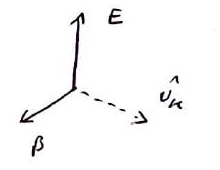
\includegraphics[width=.32\linewidth]{ottica_tex_assets/b36_p59_1.png}\end{center}
\[
n=\sqrt{\varepsilon_r\mu_r}\qquad\text{ma }\mu_r=1\text{ quasi sempre},
\qquad n=\frac cv\geq1.
\]
\[
\vv S=\frac{EB}{\mu_0}\hat u_k=\frac1{\mu_0}(\vv E\times\vv B)
\qquad\text{vettore di Poynting}.
\]
\[
p_{\mathrm{rad}}=\frac Ic(1+\eta)
\qquad\text{con }\eta\text{ coefficiente di riflessione}.
\]
\[
I=\frac P\Sigma,\qquad I=\frac12c\varepsilon_0E^2,\qquad
\varepsilon_0=8{,}85\cdot10^{-12}.
\]
% Nella pagina originale I_0 è annotato come 10^{12}, senza meno; conservato.
% Pagina originale 60
\pagina{60}
\[
P=\frac U{\Delta t}\quad\left(=\frac{\partial U}{\partial t}\right).
\]
\subsubsection*{Polarizzazione}
\[
I'=\underbrace{I\cos^2\theta}_{\text{legge di Malus}}
\quad\text{polarizzata},\qquad
I'=\frac I2\quad\text{non polarizzata}.
\]
\subsubsection*{Snell}
\[
n_1\sin\theta_1=n_2\sin\theta_2.
\]
\subsubsection*{Coefficienti di Fresnel}
\[
\chi=\frac{\cos\theta_t}{\cos\theta_i},\qquad\eta=\frac{n_2}{n_1},
\]
\[
r_\sigma=\frac{1-\eta\chi}{1+\eta\chi},\qquad
r_\pi=\frac{\chi-\eta}{\chi+\eta},\qquad
t_\sigma=\frac2{1+\eta\chi},\qquad
t_\pi=\frac2{\chi+\eta}.
\]
\subsubsection*{Angolo limite}
\[
\theta_0=\arcsin\frac{n_2}{n_1}=\arcsin\eta
\qquad\text{riflessione totale}.
\]
\subsubsection*{Angolo di Brewster}
\[
\theta_B=\arctan\eta\qquad\text{trasmissione totale}.
\]
\subsubsection*{Angolo di deviazione}
\[
\delta=i_1+i_2-\alpha.
\]
\begin{center}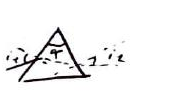
\includegraphics[width=.23\linewidth]{ottica_tex_assets/b36_p60_1.png}\end{center}
\subsubsection*{Specchio}
\[
\frac1p-\frac1q=-\frac2R,\qquad I=-\frac qp.
\]
\subsubsection*{Diottro}
\[
\frac{n_1}{p}+\frac{n_2}{q}=\frac{n_2-n_1}{R},\qquad
I=\frac{n_1}{n_2}\frac qp.
\]
\subsubsection*{Lenti}
\[
\frac1p+\frac1q=\frac1f,\qquad I=\frac qp.
\]
\[
\delta=k(r_1-r_2)=\frac{2\pi}{\lambda}d\sin\theta,
\]
\[
I_P(\theta)=I_0\left[\frac{\sin(N\delta/2)}{\sin(\delta/2)}\right]^2
\xrightarrow{N=2}I_P(\theta)=4I_0\cos^2\frac\delta2.
\]
\[
\sin\theta=m\frac\lambda d\quad\text{max principali},\qquad
\sin\theta=m'\frac\lambda{Nd}\quad\text{min},\qquad
\sin\theta=\left(m''+\frac12\right)\frac\lambda{Nd}\quad\text{max secondari}.
\]
% Pagina originale 61
\pagina{61}
\subsubsection*{Diffrazione}
\[
I_P=I_{\max}\left[\frac{\sin(\frac\pi\lambda a\sin\theta)}
{\frac\pi\lambda a\sin\theta}\right]^2.
\]
Massimo visibile: $\sin\theta=1$ ($\theta=\pi/2$).
\subsubsection*{Interferenza e diffrazione}
\[
I_P=I_{\max}
\underbrace{\left(\frac{\sin(\frac\pi\lambda a\sin\theta)}
{\frac\pi\lambda a\sin\theta}\right)^2}_{\text{diffrazione}}
\underbrace{\left(\frac{\sin(\frac\pi\lambda Nd\sin\theta)}
{\sin(\frac\pi\lambda d\sin\theta)}\right)^2}_{\text{interferenza}}.
\]
\[
\sin\theta=m\frac\lambda d<\frac\lambda a
\quad\Longrightarrow\quad m<\frac da\qquad\text{per essere visibile}.
\]

\end{document}
